% Estructura obligatoria: títulos y orden de las bases.
% El catálogo detallado pertenece al SD2; T-12 se entrega como archivo propio.
\chapter{Introducción al Alcance de la Solución}

Este capítulo formaliza la frontera contractual, técnica y operacional de la solución provista por Synaptix para Marina y Club Náutico Bahía Panitao S.A., delimitando con precisión los compromisos de entrega por etapa y su correspondencia. El alcance traduce directamente el diagnóstico: custodia rigurosa de embarcaciones, seguridad de la vida humana en el agua, trazabilidad de faenas en varadero, acreditación de contratistas, cumplimiento ambiental para la temporada 2029 y erradicación de la dispersión de registros en papel y planillas aisladas \parencite[caps.~3, 7 y 10]{caso07}. 
La propuesta articula armónicamente el alcance del producto con el alcance del proyecto a lo largo de un ciclo contractual de 56 meses, integrando como componentes nativos de la solución cinco innovaciones. La trazabilidad completa de los 146 requerimientos funcionales, 56 requerimientos no funcionales y 374 requisitos técnicos transversales se acredita código por código en el \ReferenciaAnexo{Formulario T-12}{SYNAPTIX-Formulario-T-12.pdf}.

\newpage

\section{Resumen Ejecutivo de la Solución}
Synaptix propone para la Marina y Club Náutico Bahía Panitao S.A. una plataforma digital unificada que centraliza los registros operacionales y conserva la trazabilidad de los hechos que intervienen en la operación marítima, la custodia patrimonial, el mantenimiento logístico y el cumplimiento normativo. La solución sustituye la fragmentación actual por procesos estandarizados y auditables, diseñados a la medida de las condiciones climáticas y operacionales extremas del Seno de Reloncaví.
\begin{resumenejecutivo}
La solución se estructura en dos etapas de proyecto seguidas de una fase de operación continua:
\begin{itemize}
    \item \textbf{Etapa 1 (Meses 1 al 16):} Entrega el núcleo crítico de seguridad humana y custodia (salidas y regresos, alertas tempranas de marejada por tres canales simultáneos, control escolar de vela con bloqueo atómico en rampa, inventario de amarras y telemetría horaria de torretas), garantizando al menos 24 horas continuas de operación desconectada en el recinto mediante el Nodo de Borde (NBR). La captura de consumos de agua y energía se habilita en E1 mediante la asociación de medidores y amarras, la validación de lecturas y su conservación y consulta. Las comprobaciones de instalación e integración preceden a la incorporación de los registros a la serie validada, porque los indicadores ambientales requieren antecedentes trazables anteriores a la temporada 2029 \parencite[sec.~13.2; cap.~15, RT-05.10]{caso07}.
    \item \textbf{Etapa 2 (Meses 13 al 21):} Desplegada en solapamiento controlado, completa la logística de varadero y travelift con modo pasivo de maniobra, acreditación de contratistas por código QR, cadena de custodia de residuos peligrosos (RESPEL) integrada a SIDREP, motor de hechos facturables hacia el ERP contable y expedientes digitales para las 14 naves en abandono.
    \item \textbf{Fase de Operación (Meses 21 al 56):} El servicio gestionado (MSP) comprende la administración de la infraestructura híbrida y el soporte técnico durante 36 meses bajo marco ITIL 4, atendiendo a una organización sin dotación TI interna. Este servicio obligatorio se distingue de IN-04, cuyo incentivo adicional depende de resultados comprobados y aceptados.
\end{itemize}
El software asiste y registra, pero no usurpa potestades privativas: DIRECTEMAR conserva el otorgamiento legal del zarpe y el ERP contable vigente mantiene la emisión de documentos tributarios \parencites[art.~16, pp.~11--12]{bases-admin}[caps.~10 y 13]{caso07}.
\end{resumenejecutivo}

\subsection{Propuesta de Valor y Visión Operacional Integral}
La propuesta de valor de Synaptix radica en establecer una cadena probatoria y operativa continua de extremo a extremo: cada hecho capturado en terreno se asocia de forma determinista con el operador o dispositivo que lo originó, la validación de seguridad previa, la evidencia física conservada y su impacto comercial o ambiental posterior. De este modo, una recalada de visitante se enlaza automáticamente con la verificación dimensional de la amarra, la telemetría horaria de consumos y la transferencia del lote facturable al sistema contable; asimismo, una intervención en varadero relaciona al contratista acreditado, la inspección fotográfica previa del casco, el plan de eslingado del travelift y la custodia de los residuos peligrosos generados.
Esta visión se materializa incorporando dentro del alcance del producto las cinco innovaciones obligatorias del Artículo 28° de las Bases Administrativas (Subdocumento 13), diseñadas específicamente para resolver los dolores diagnosticados en el Capítulo 2 que no están propuestos como base:
\begin{enumerate}
    \item \textbf{Innovación 1: Servicio de Solicitud y Seguimiento
    de Mantenimiento de Embarcaciones (Producto/Servicio):}
    Servicio mediante el cual el armador presenta una solicitud
    de mantenimiento y consulta su estado. La marina revisa y deriva
    la solicitud al contratista pertinente, quien registra su aceptación
    o rechazo, avance y finalización. Se integra con AUT para la
    interacción de los usuarios, CTR para verificar la habilitación
    del contratista, VAR para vincular la orden de trabajo y ALE
    para comunicar cambios de estado. La aceptación de la solicitud
    no autoriza por sí sola el acceso a la faena, y el cierre
    administrativo no certifica la calidad técnica de la reparación.

    \item \textbf{Innovación 2: Programa de Mantenimiento Preventivo
    en Invernada (Proceso):}
    Organización de un ciclo de mantenimiento preventivo durante
    la permanencia de las embarcaciones en seco. A partir de una
    ficha de ingreso y un catálogo de tareas, se presentan propuestas
    que el armador puede aceptar o rechazar. La marina distribuye
    los trabajos aceptados considerando las fechas de botadura,
    las posiciones en la explanada y la disponibilidad de recursos
    y contratistas habilitados. Cada trabajo se vincula con una
    solicitud de la innovación 1 para registrar su avance; antes
    de la botadura se revisan los pendientes y se comunican los
    ajustes necesarios. El programa reutiliza VAR, CTR, AUT, ALE
    y ADM, sin duplicar la agenda del varadero.
    
    \item \textbf{Innovación 3: Lectura inteligente de documentos para el ingreso asistido de antecedentes (Tecnológica):} Extracción asistida mediante Amazon Textract y reglas de comprobación, aplicada inicialmente a pólizas de embarcaciones. El sistema propone campos y conserva el documento original; un funcionario autorizado revisa, corrige y confirma los antecedentes antes de incorporarlos al expediente. No acredita autenticidad ni cobertura y mantiene el ingreso manual como alternativa ante errores o indisponibilidad.

    \item \textbf{Innovación 4: Servicio Gestionado por Resultados (Modelo de negocio o de contratación):} Mecanismo que vincula una parte variable de la remuneración operacional a la reducción comprobada del tiempo activo de coordinación de solicitudes del servicio adicional IN-01. El reconocimiento requiere datos comparables, condiciones de calidad y evidencia aceptada; no remunera nuevamente la implementación obligatoria ni sustituye los compromisos propios de mesa de ayuda, seguridad, continuidad y disponibilidad. El beneficio de IN-01 no se contabiliza dos veces.

    \item \textbf{Innovación 5: Pasaporte Ambiental Náutico con Planes de Reducción (Experiencia de usuario, sostenibilidad o impacto social):} Historial propio y plan voluntario de acciones para reducir el agua suministrada en la marina por día efectivo de permanencia de las embarcaciones participantes. Cada acción conserva responsable, plazo, evidencia y evaluación posterior. Reutiliza la medición individual y las permanencias validadas, sin modificar cobros ni actuar automáticamente sobre el suministro. No sustituye la trazabilidad obligatoria de consumos, residuos y capacitación ni certifica ambientalmente una embarcación o la marina.
\end{enumerate}

La solución respeta los límites institucionales y materiales: la plataforma no otorga zarpes oficiales, atribución de la Capitanía de Puerto; no emite facturas ni documentos fiscales, función del ERP contable; y no ejecuta labores de búsqueda y salvamento marítimo (SAR). No administra la operación ni el punto de venta del restaurante, pero registra su relación contractual y sus consumos de servicios de la marina. Tampoco aplica automáticamente restricciones de acceso a una embarcación por morosidad: una medida de cobranza que afecte ese acceso requiere decisión formal de la compañía, registrada y fundamentada.

\subsection{Ciclo de Vida Contractual, Etapas y Modelo de Servicio Gestionado}
Se distingue formalmente el \textbf{alcance del producto} (las funcionalidades, interfaces, subsistemas y servicios provistos por la plataforma) del \textbf{alcance del proyecto} (el esfuerzo temporal de ingeniería, migración, pruebas de carga, implantación, capacitación y marcha blanca necesario para materializarlo). El contrato contempla un ciclo total de 56 meses, estructurado en dos etapas sucesivas con solapamiento controlado y una fase final de régimen operacional:

\begin{figure}[H]
    \centering
    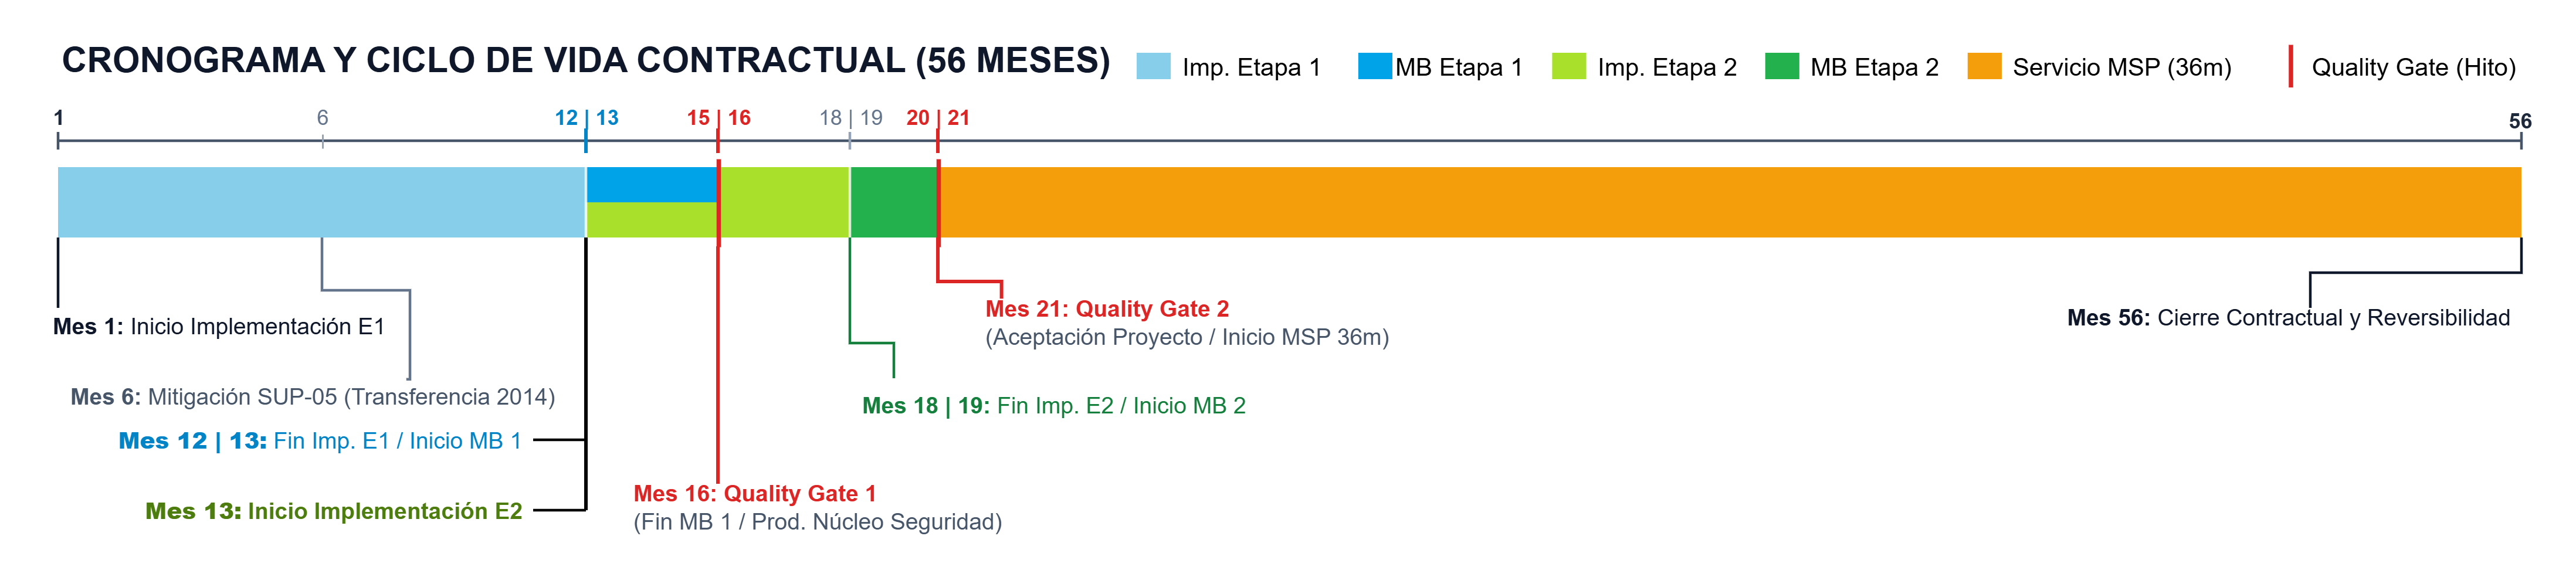
\includegraphics[width=\textwidth]{figuras/timeline-hitos.png}
    \caption{Ciclo de vida contractual, hitos de control, compuertas de calidad y servicio gestionado}
    \label{fig:ciclo_vida_contractual}
    \FuenteTabla{elaboración propia}
\end{figure}

Como ilustra la Figura~\ref{fig:ciclo_vida_contractual}, el cronograma desacopla los riesgos técnicos y operacionales en tres fases claramente delimitadas:
\subsubsection{Etapa 1: Núcleo de Seguridad y Continuidad Operacional (Meses 1 al 16)}
Esta etapa concentra los procesos de misión crítica vinculados a la salvaguarda de la vida humana, la custodia náutica y la continuidad del recinto portuario:
\begin{itemize}
    \item \textbf{Fase de Implementación (Meses 1 al 12):} Comprende la ingeniería de detalle de ocho capas (ISO/IEC/IEEE 42010), el despliegue de la infraestructura en nube (AWS Santiago), el aprovisionamiento del Nodo de Borde en Recinto (NBR) en gabinete estanco IP55 y la construcción de los módulos esenciales de operación:
    \begin{itemize}
        \item \emph{Entregable E1.1 (Especificación y Gobernanza):} Documento de arquitectura, catálogo formal de datos, especificaciones de interfaz (OpenAPI 3.1 / AsyncAPI 2.6) y protocolos de prueba de aceptación.
        \item \emph{Entregable E1.2 (Infraestructura Híbrida y Borde):} Despliegue de los clústeres elásticos en AWS, aprovisionamiento de los dos nodos del NBR con persistencia local en PostgreSQL Edge y SQLite Outbox, y configuración del canal seguro mTLS.
        \item \emph{Entregable E1.3 (Módulos Críticos de Operación):} Construcción y puesta a punto de los componentes esenciales: Navegación, Salidas y Zarpes (\textbf{NAV}); Alertas Tempranas de Marejada multicanal (\textbf{ALE}); Escuela de Vela y Protección de Menores (\textbf{ESC}); Gestión básica y compatibilidad física de Amarras (\textbf{AMA}); Despacho local de Combustible y Colector de Telemetría horaria de torretas (\textbf{CON}); Inventario de Fondeos, Inspecciones desconectadas y Piloto Sensórico en Bahía Ilque (\textbf{BOY}); Núcleo de Datos Maestros y Auditoría (\textbf{ADM}); y Portales iniciales de autoatención para planes de navegación (\textbf{AUT}).
        \item \emph{Entregable E1.4 (Migración Inicial de Datos):} Extracción, perfilado, saneamiento trazable y carga de la totalidad del padrón de socios y armadores, de los contratos de amarra vigentes con su documentación asociada y del registro de embarcaciones. Se incorporará la matrícula de la escuela de vela de los últimos tres años. Esta distribución habilita la identificación, asignación de amarras, navegación y control escolar requeridos por E1. El plan de migración conservará la relación entre cada registro de destino y su fuente, y documentará los defectos detectados y las decisiones de tratamiento, sin eliminar antecedentes obligatorios
        \parencite[cap.~15, RT-05.15]{caso07}.
    \end{itemize}
    \item \textbf{Hito de Contingencia Temprana (Mes 6):} La transferencia documentada del conocimiento del sistema administrativo de 2014 comienza en el mes 6. Sus entregables son los procedimientos de extracción, el inventario de fuentes, la matriz de transformación de saldos y el resultado de un simulacro de cierre y conciliación. Esta anticipación reduce la dependencia de la única persona que conoce el sistema de origen y permite detectar errores antes de los ensayos completos de migración. El acceso a las fuentes se gestiona conforme a SUP-02 \parencite[cap.~15, RT-05.15]{caso07}.
    \item \textbf{Fase de Implantación y Marcha Blanca (Meses 13 al 15):} Tres meses de operación supervisada con datos y usuarios reales, en convivencia con los registros vigentes y con medición de los indicadores de E1. La capacitación y las intervenciones respetan el congelamiento del 15 de diciembre al 15 de marzo, las campañas de varada y botadura en lo que afecte al varadero y las 14 fechas del calendario náutico. Los avisos de marejadas suspenden las actividades programadas; la planificación absorbe esas interrupciones sin desplazar los hitos contractuales. Durante este período se comprueban los procesos críticos, la conciliación y la preparación del personal para el paso a producción \parencite[cap.~10; cap.~15, RT-10.05]{caso07}.
    \item \textbf{Paso a Producción y Quality Gate 1 (Mes 16):} Formalizado mediante el \emph{Entregable E1.5 (Acta de Cierre de Marcha Blanca y Certificación)}. Requiere la aceptación de CA-01 a CA-08, CA-10, CA-13 y CA-23; la verificación de captura y consulta individual de CA-18; y el registro operacional e historial de inspección de CA-20. La continuidad y operabilidad de CA-25 se verifican para el alcance de E1. Esta distribución permite recibir las capacidades operacionales de la primera etapa y comprobar sus dependencias de medición y continuidad. El expediente reúne los resultados de estos criterios y las seis condiciones de cierre de marcha blanca; la Contraparte Técnica suscribe el acta correspondiente. El alcance de E1 comprende la habilitación de la captura y conservación de consumos para construir la serie ambiental anterior a la temporada 2029. El registro de puesta en servicio identifica su fecha, los puntos habilitados, las lecturas recibidas y las incidencias de captura, permitiendo demostrar la cobertura temporal efectiva. Las series de consumo se conservan durante cinco años, conforme a RT-05.10 del Caso 07 \parencite[sec.~13.2; cap.~15, RT-05.10]{caso07}.
\end{itemize}

\subsubsection{Etapa 2: Automatización Logística, Gestión Ambiental y Cierre Administrativo (Meses 13 al 21)}
Se ejecuta en solapamiento controlado con la estabilización de la primera etapa, incorporando las capacidades comerciales, analíticas, logísticas y ambientales sobre datos maestros ya consolidados:
\begin{itemize}
    \item \textbf{Fase de Implementación (Meses 13 al 18):} Construcción de los módulos avanzados:
    \begin{itemize}
        \item \emph{Entregable E2.1 (Varadero, Logística y Medio Ambiente):} Módulo de Varadero, Travelift e Invernada con Ficha Técnica de Izaje en modo pasivo y reprogramación ante temporales (\textbf{VAR}); Control de Acceso y Acreditación de Contratistas mediante códigos QR en portería (\textbf{CTR}); Trazabilidad integral de Residuos Peligrosos RESPEL y enlace con SIDREP (\textbf{AMB}); y evaluación de la ampliación sensórica en Bahía Ilque (\textbf{BOY}) condicionada a los resultados del piloto de E1 (DEC-19).

        La incorporación de las cinco innovaciones definidas en el Subdocumento 13 complementa las capacidades obligatorias de la plataforma. A continuación se delimita el aporte de cada una, sus dependencias y su calendario de preparación técnica, separando estas actividades de los pilotos y de la materialización operativa descritos posteriormente.

        \textbf{IN-01: Servicio de Solicitud y Seguimiento de Mantenimiento de Embarcaciones} permite al armador presentar solicitudes, a la marina revisarlas y derivarlas, y al contratista registrar aceptación o rechazo, avance y finalización. El diseño se realiza en los meses 13--14, la construcción e integración en 14--15 y las pruebas en el mes 16. Utiliza \textbf{AUT}, \textbf{CTR}, \textbf{VAR}, \textbf{ADM} y \textbf{ALE}, manteniendo independientes la aceptación de la solicitud, la autorización de acceso y la orden de trabajo de la solución base.

        \textbf{IN-02: Programa de Mantenimiento Preventivo en Invernada} organiza las tareas aceptadas por el armador según posiciones en la explanada, fechas de botadura y disponibilidad de recursos y contratistas habilitados. Reutiliza IN-01 y los módulos \textbf{VAR}, \textbf{CTR}, \textbf{AUT}, \textbf{ALE} y \textbf{ADM}, sin duplicar la agenda del varadero. Su diseño comprende los meses 13--14; la ficha y las propuestas, 14--15; el calendario y la integración, 15--16; y las pruebas y aceptación técnica, 16--17. La comprobación del beneficio conserva su ventana estacional.

        \textbf{IN-03: Lectura inteligente de documentos para el ingreso asistido de antecedentes} comprende diseño en los meses 13--14, configuración de extracción en 14, revisión e integración en 15 y pruebas y preparación en 16. Su incorporación requiere las interfaces de \textbf{AUT}, \textbf{ADM} y \textbf{NAV}, el repositorio, la auditoría y los controles de IA definidos para la revisión humana de pólizas.

        \textbf{IN-04: Servicio Gestionado por Resultados} comprende la definición de la regla comercial y de medición en los meses 2--4, instrumentación y expediente en 13--15 y pruebas en 16. La medición utiliza el flujo adicional de IN-01 y distingue el tiempo activo de coordinación de la espera de respuesta del contratista.

        \textbf{IN-05: Pasaporte Ambiental Náutico con Planes de Reducción} comprende diseño del plan, consentimiento y reglas en los meses 13--14, historial y portal en 14--15 y pruebas funcionales y de seguridad en 16. Su evaluación utiliza mediciones individuales validadas, asociaciones vigentes entre amarra y embarcación y permanencias conciliadas.
        \item \emph{Entregable E2.2 (Motor Financiero y Automatización Comercial):} Algoritmo determinista de asignación y gestión de Lista de Espera (\textbf{AMA}); Transformación de consumos medidos en hechos facturables validados bajo UUIDv4 (\textbf{CON}); Motor consolidado de Hechos Facturables, tramos de mora sin restricciones automáticas de acceso por deuda, con registro de las decisiones formales y fundamentadas de la compañía para las medidas excepcionales, y Expediente Forense Digital PDF/A para las 14 embarcaciones en abandono (\textbf{FAC}); y adaptadores de enlace con el ERP contable (INT-01).
        \item \emph{Entregable E2.3 (Portales Web Completos e Interoperabilidad):} Suite integral de Portales de Autoatención (\textbf{AUT}) para armadores socios, apoderados, visitas (con pasarela de pago digital) y contratistas; e interfaz con torniquetes físicos en portería (INT-05).
    \end{itemize}
    \item \textbf{Fase de Implantación y Marcha Blanca Integral (Meses 19 y 20):} Dos meses de operación supervisada, con simulación masiva de cobranza, maniobras asistidas de izaje, conciliación de datos y preparación del corte del sistema administrativo de 2014. La migración se completa con la historia de pagos y saldos de seis años, la totalidad de los antecedentes de las 14 embarcaciones abandonadas y la totalidad del registro de invernadas. Estos conjuntos habilitan la gestión financiera, la custodia probatoria y las operaciones de varadero de E2. Se verificarán además la integridad y continuidad de los conjuntos incorporados en E1 y las modificaciones producidas desde su carga.
    
    Los antecedentes históricos adicionales a los conjuntos obligatorios permanecerán consultables en un repositorio verificable, con integridad y acceso restringido durante su retención aplicable. Este repositorio complementa la migración obligatoria y no la sustituye. La transferencia comprende datos y antecedentes; la consulta histórica se mantiene sin exigir la continuidad operativa del software sin soporte. El corte definitivo queda sujeto al cierre y aceptación de la marcha blanca \parencite[cap.~15, RT-05.10 y RT-05.15]{caso07}.

    El plan conjunto de migración identificará alcance, origen, volumen, reglas de transformación, criterios de calidad, estrategia de ejecución y plan de reversión, conforme a RT-05.11 a RT-05.14 de las Bases Técnicas Transversales. La ejecución comprenderá perfilado y saneamiento previo, con informe de defectos y decisiones de tratamiento, y al menos dos ensayos completos sobre Preproducción antes de la migración definitiva. Cada ensayo registrará el tiempo total y el resultado de la conciliación mediante recuentos, sumas de control y muestreo dirigido. Toda diferencia quedará explicada y se comprobará el procedimiento de reversión. La distribución por etapas mantendrá disponibles los antecedentes necesarios para E1 y completará los seis conjuntos obligatorios antes del corte definitivo de E2.

    Durante la marcha blanca se ejecutan las verificaciones de migración, conciliación y reversión y se prepara el corte definitivo. Para proteger la continuidad operacional y evitar una sustitución sin aceptación formal, el sistema administrativo de 2014 será reemplazado operacionalmente únicamente después del cierre satisfactorio de la marcha blanca y de la suscripción del acta E2.4 por la Contraparte Técnica. Se preservarán la consulta de los antecedentes históricos y la continuidad del alcance de E1.

    Los pilotos adicionales se distinguen de la marcha blanca obligatoria de la plataforma. En \textbf{IN-01}, la línea base se levanta en el mes 18 con el flujo adicional desactivado para la cohorte evaluada; la capacitación se realiza al finalizar esa medición y el piloto se ejecuta y evalúa en el mes 19. \textbf{IN-04} utiliza los meses 18--19 para comparar el esfuerzo activo de coordinación, sin pagos variables durante el piloto. \textbf{IN-03} compara ingreso manual y asistido durante ocho semanas consecutivas dentro de los meses 18--19. \textbf{IN-05} compara 28 días del mes 18 con 28 días del mes 19, aplicando las acciones entre ambas ventanas. Los protocolos, muestras y metas de evaluación se desarrollan en el Subdocumento 13.

    Para \textbf{IN-02}, $M_{\mathrm{inv}}$ corresponde al primer junio disponible con IN-01 y sus interfaces aceptadas, no anterior al mes 21. El piloto comprende junio--agosto, desde $M_{\mathrm{inv}}$ hasta $M_{\mathrm{inv}}+2$; los resultados se observan durante las botaduras hasta $M_{\mathrm{inv}}+5$ y se consolidan con la evaluación y transferencia en $M_{\mathrm{inv}}+6$. El ciclo completo, incluida la recepción de abril--mayo, se aplica desde $M_{\mathrm{inv}}+10$ cuando el plazo contractual permite concluir su evaluación. Estas ventanas se vinculan a la fecha de inicio contractual y respetan las restricciones operacionales sin desplazar hitos.
    \item \textbf{Paso a Producción y Quality Gate 2 (Mes 21):} Formalizado mediante el \emph{Entregable E2.4 (Acta de Aceptación Definitiva de la Plataforma)}, acreditando la aceptación de CA-09, CA-11, CA-12, CA-14 a CA-17, CA-21, CA-22 y CA-24; la integración de CA-18 con facturación e indicadores ambientales; la continuidad de CA-20; y la preparación integral del servicio de CA-25. Esta recepción comprueba la integración del alcance completo, sin degradar las capacidades, disponibilidad ni integridad de los datos de E1. El expediente incorpora la evidencia técnica de CA-19 correspondiente a esta recepción y su trazabilidad hacia el cierre ambiental exigido antes de la temporada 2029. La Contraparte Técnica suscribe el acta una vez satisfechas las seis condiciones de cierre. La materialización operativa de \textbf{IN-01}, \textbf{IN-03}, \textbf{IN-04} e \textbf{IN-05} corresponde al mes 21, tras las pruebas, pilotos y aceptaciones respectivos. En \textbf{IN-02}, la aceptación técnica de la capacidad incorporada se distingue de la comprobación de su beneficio estacional: piloto, informe y transferencia conservan la ventana definida en el Subdocumento 13, sin alterar los hitos de recepción.
\end{itemize}

\subsubsection{Fase de Operación Continua y Servicio Gestionado (Meses 21 al 56)}
Aprobada la recepción definitiva de la Etapa 2, inicia el régimen de operación continua por 36 meses mediante el servicio gestionado (MSP). IN-04 añade un mecanismo de remuneración variable por resultados de coordinación, conservando independientes las obligaciones de soporte, seguridad, continuidad y disponibilidad. La ausencia de un área TI interna en la marina determina el siguiente reparto entre autoridad de negocio y responsabilidad técnica:
\begin{itemize}
    \item \textbf{Decisiones de Negocio y Participación del Cliente:} Los responsables de procesos de la marina aprueban tarifas, reglas de asignación, excepciones operacionales y medidas de cobranza conforme a sus atribuciones. Participan en las pruebas, la capacitación, la revisión de entregables y las actas correspondientes. El servicio gestionado ejecuta la administración funcional, aplica las configuraciones autorizadas y proporciona soporte a las personas usuarias. Las funciones de aprobación se documentan con titular, suplente, atribuciones y acceso individual, para mantener la continuidad durante vacaciones, licencias y rotación sin requerir un cargo informático del cliente.
    \item \textbf{Servicio Gestionado por Synaptix (MSP):} El Gerente de Servicio conduce la prestación y responde por la coordinación de la administración técnica y funcional. El alcance comprende identidades y accesos, aplicación de parámetros de negocio autorizados, respaldos y restauración, cambios de producción, mantenimiento del software y soporte funcional, con participación de especialistas de NOC, SOC e infraestructura. Los procedimientos y registros distinguen la aprobación de una regla por el cliente de su aplicación y verificación por el servicio. Esta separación conserva la autoridad del mandante y concentra la ejecución especializada en el adjudicatario. La prestación incluye:
    \begin{itemize}
        \item \emph{Mesa de Ayuda Bilingüe Estacional:} Atención en español e inglés todos los días, de 06:00 a 24:00 durante la temporada alta del 15 de noviembre al 31 de marzo, y de 08:00 a 20:00 el resto del año. El centro cumplirá los indicadores de atención establecidos en las Bases Técnicas Transversales: 80\,\% de las atenciones antes de 20 segundos, resolución al primer contacto de al menos 70\,\% y tasa de abandono no superior al 5\,\%. La temporada de atención se distingue del congelamiento de intervenciones del 15 de diciembre al 15 de marzo.
        \item \emph{Canal Permanente $24/7/365$:} El canal de notificación de emergencia y la recepción de alertas por planes de navegación vencidos operan sin excepción durante todo el año. La atención de incidentes críticos y altos mantiene igualmente cobertura $24/7/365$, independiente del horario de la mesa estacional. Cada evento conserva su clasificación, responsable, actuaciones y escalamiento. Esta cobertura asegura que el cierre de la atención ordinaria no interrumpa los procesos de emergencia ni la respuesta a incidentes de mayor severidad.
        \item \emph{Observabilidad Proactiva y SLAs:} Monitoreo unificado con OpenTelemetry, respaldo inmutable 3-2-1-1-0 en AWS S3 Object Lock, mantención correctiva/evolutiva, traslados marítimos periódicos a Bahía Ilque y cumplimiento del compromiso de disponibilidad del 99,9\,\%, garantizando la sostenibilidad total del criterio CA-25.
        \item \emph{Registro y Escalamiento del Soporte:} El canal único de registro reúne incidentes y solicitudes con número de ticket, clasificación por severidad y seguimiento hasta el cierre conforme. El nivel 1 recibe, clasifica, resuelve consultas básicas y deriva; el nivel 2 realiza diagnóstico, configuración y soporte especializado; el nivel 3 aborda problemas nuevos y resolución experta. Los especialistas de niveles 2 y 3 se trasladan al sitio cuando la resolución lo requiere, por el medio más rápido disponible y sin degradar la atención de los demás sitios. El soporte del fabricante se gestiona como nivel 4, manteniendo la responsabilidad del adjudicatario frente al cliente. Los procedimientos propios del negocio y las aplicaciones del cliente no provistas por el servicio conservan la responsabilidad establecida en las Bases Técnicas Transversales.
        \item \emph{Transferencia y Continuidad de Funciones:} La documentación operacional, la capacitación práctica y la autoformación en línea con registro de avance permiten ejecutar los procedimientos asignados al cliente y utilizar los canales de soporte. El registro de funciones identifica titulares, suplentes y accesos; las pruebas comprueban la ejecución por el suplente ante ausencia del titular. La transferencia prepara a las personas para sus funciones operacionales y de aprobación, sin desplazarles la administración técnica ni el mantenimiento del software.
        \item \emph{Reporte y Evidencia del Servicio:} Los datos de observabilidad estarán disponibles para el cliente en tiempo real y serán exportables. Dentro de los primeros cinco días hábiles de cada mes se entregará el informe de niveles de servicio, con indicadores, incidentes del período, causas raíz y plan de acción. El histórico de soporte y su análisis mensual alimentarán la base de conocimiento y las acciones de mejora, permitiendo comprobar el cumplimiento y corregir problemas recurrentes.
    \end{itemize}

    El seguimiento de \textbf{IN-01}, la operación del ingreso documental asistido de \textbf{IN-03} y el seguimiento del plan ambiental de \textbf{IN-05} continúan desde el mes 21 hasta el 56. En \textbf{IN-04}, la conciliación mensual reconoce únicamente resultados con evidencia y condiciones aceptadas; cuando la evidencia es insuficiente, el componente variable del período es cero y se mantienen las obligaciones del servicio. \textbf{IN-02} opera incrementalmente desde $M_{\mathrm{inv}}$ hasta el término contractual, con evaluación y transferencia en su ventana estacional y vinculación al flujo de solicitudes de IN-01.
\end{itemize}

\newpage

\section{Alcance}

Esta sección establece las capacidades, servicios y límites contractuales de la solución propuesta por Synaptix para Marina y Club Náutico Bahía Panitao S.A. Se descompone la complejidad operacional del puerto en componentes manejables, organizados en dos etapas sucesivas de implementación y una fase de servicio gestionado continuo por 36 meses. La delimitación formal de responsabilidades fija con precisión qué entrega el proponente, qué adquisiciones y obras corresponden al mandante, y qué funciones permanecen bajo la potestad exclusiva de autoridades del Estado y terceros.

\subsection{Reparto entre Etapas y Criterios de Asignación Operacional}

La asignación de capacidades entre la Etapa 1 (E1) y la Etapa 2 (E2) responde a criterios objetivos de criticidad de la vida humana, mitigación de riesgos náuticos inmediatos, requerimientos regulatorios ambientales externos y capacidad de absorción del personal del puerto. La Figura~\ref{fig:capability_map} sintetiza el Mapa de Capacidades del Negocio (\emph{Capability Map}) organizado cronológica y funcionalmente de izquierda a derecha.

\begin{figure}[H]
    \centering
    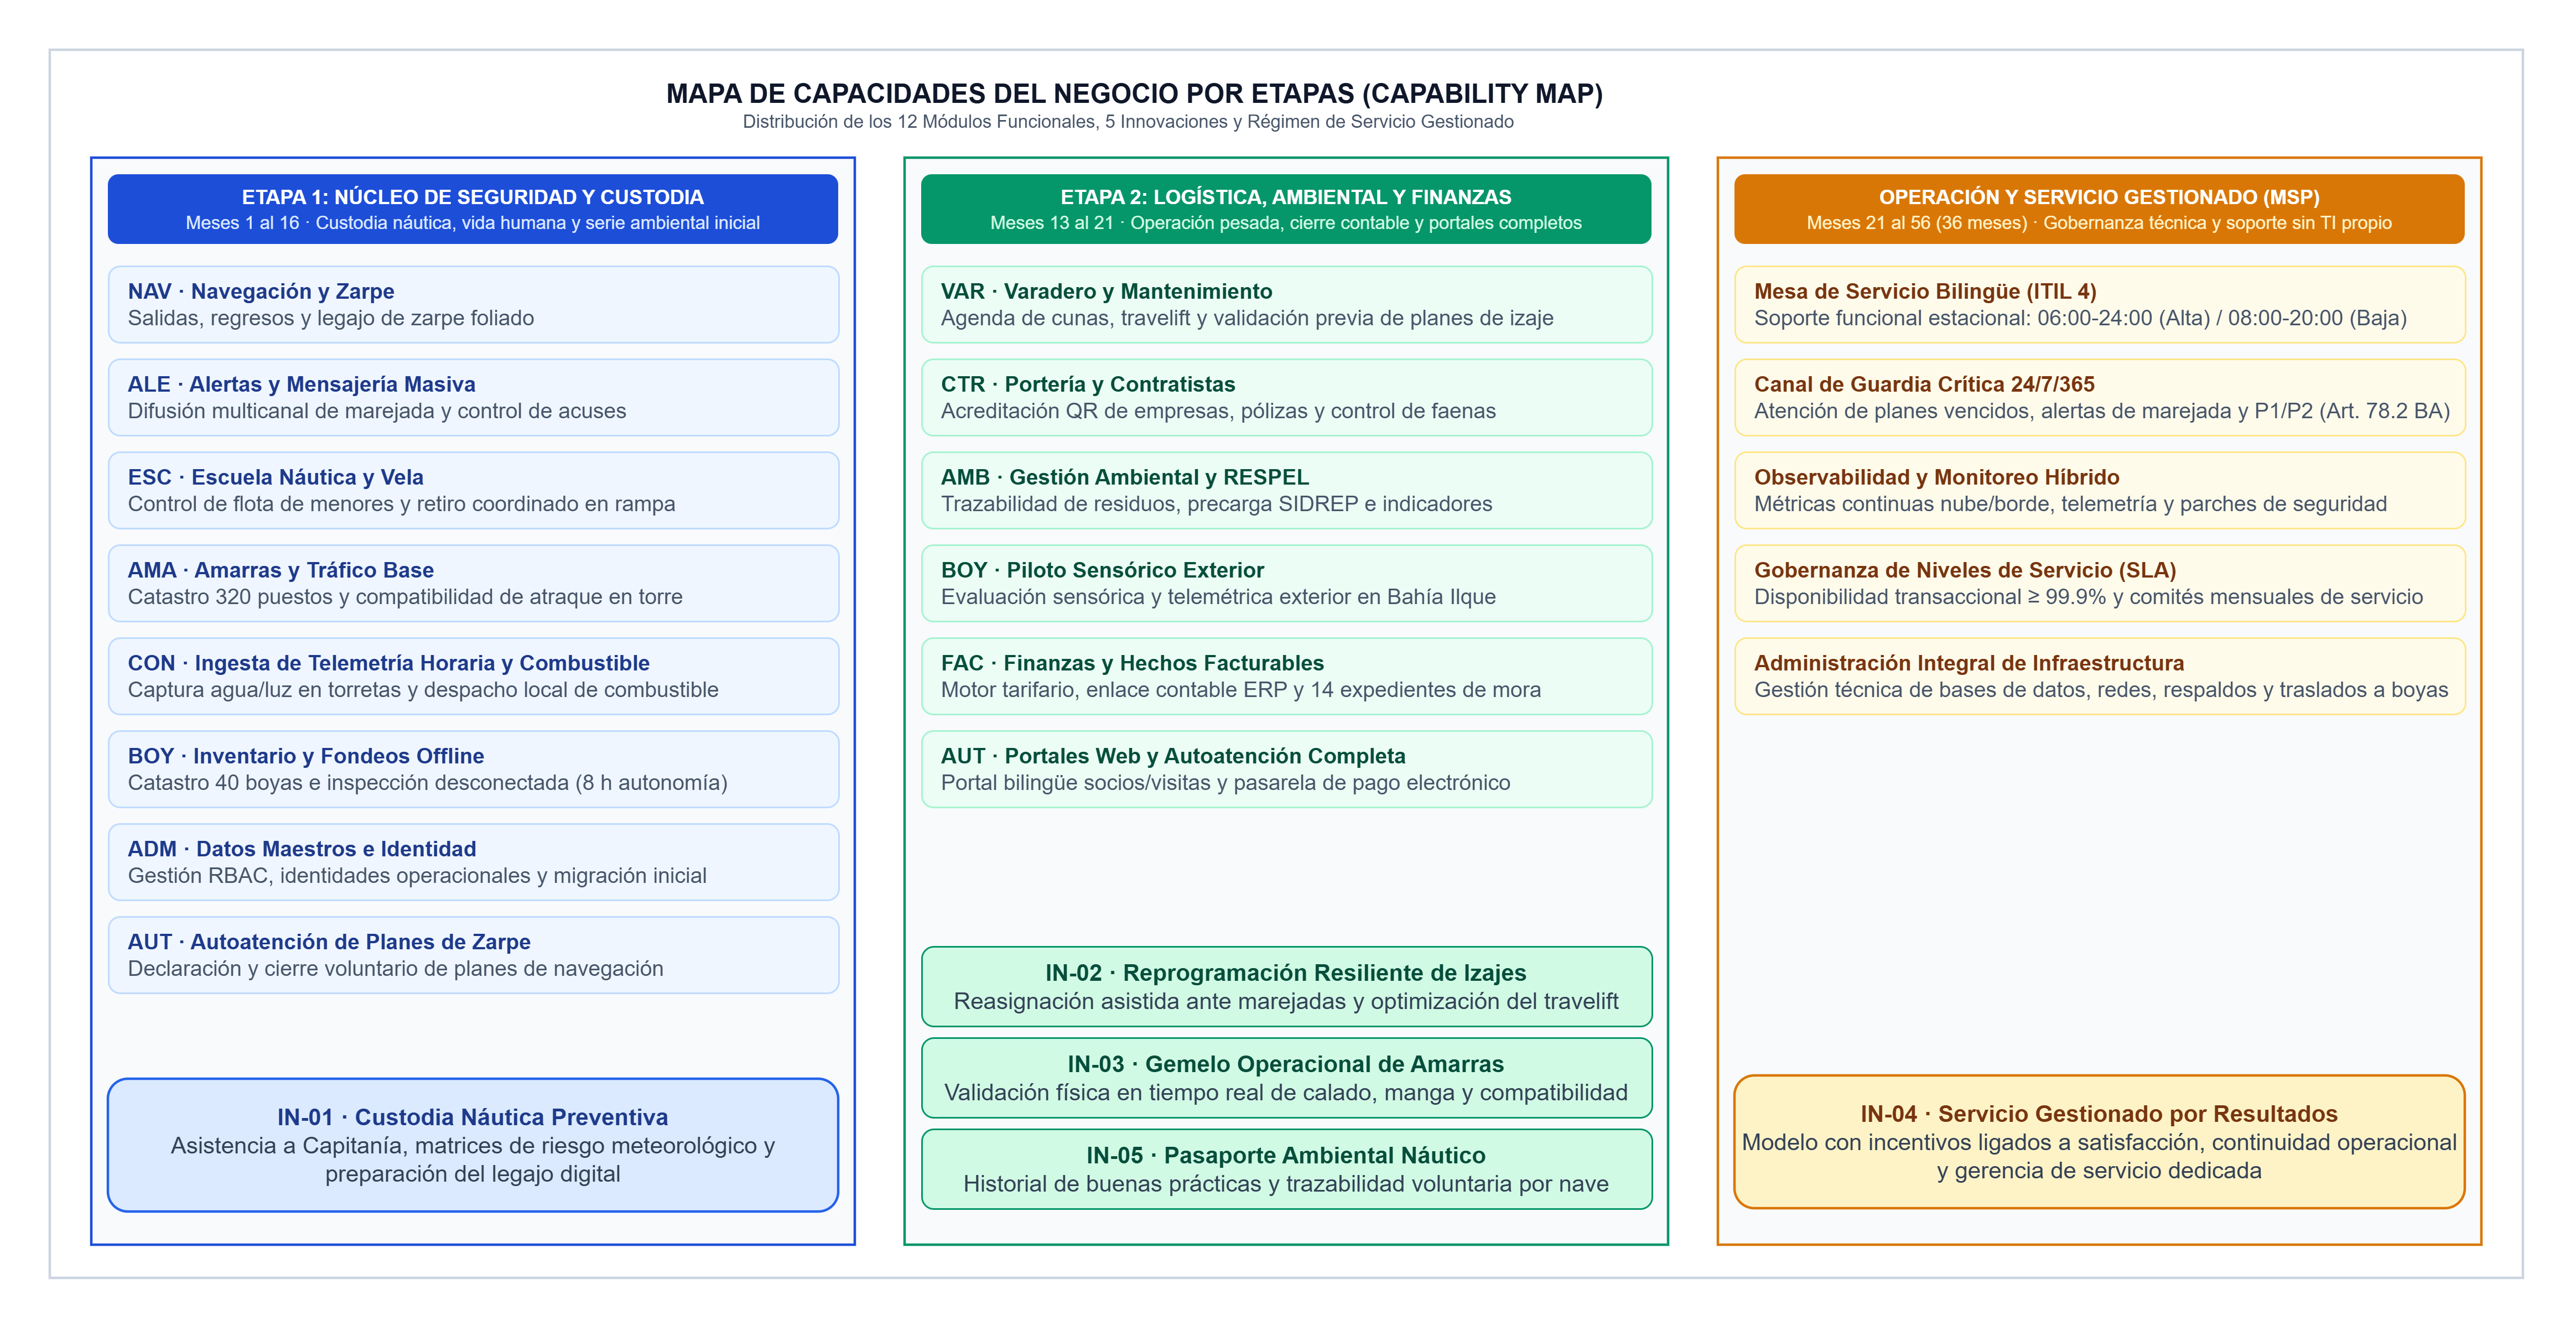
\includegraphics[width=\textwidth]{figuras/mapa-capacidades.png}
    \caption{Mapa de capacidades del negocio por etapas y fases operacionales (Capability Map)}
    \label{fig:capability_map}
    \FuenteTabla{elaboración propia}
\end{figure}

El criterio rector de asignación operacional se articula en tres grandes fases secuenciales:

\begin{enumerate}
    \item \textbf{Etapa 1 --- Núcleo de Seguridad, Custodia y Continuidad (Meses 1 al 16):} Prioriza la protección de la vida humana y la trazabilidad de naves en agua. Incorpora los módulos de Operación marítima y zarpe (\texttt{NAV}), Alertas y comunicaciones masivas (\texttt{ALE}), Escuela náutica de menores (\texttt{ESC}), Amarras base (\texttt{AMA}), Ingesta de telemetría horaria (\texttt{CON}), Boyas e inspección desconectada (\texttt{BOY}), Datos maestros y perfiles (\texttt{ADM}) y Autoatención básica de planes de navegación (\texttt{AUT}). Estas capacidades corresponden a la solución base.
    
    En esta etapa rige la resolución de la decisión técnica \textbf{DEC-01}: la confirmación de ocupación de las 320 amarras de atraque no se supedita a sensores inalámbricos en agua, sino a la correlación estricta entre la bitácora operacional de zarpe/retorno y la ronda física obligatoria de marinería registrada en tablets de 10'' fuera de cobertura (\emph{Modo Cubierta}). La integración de los 640 medidores en E1 comprende captura horaria, asociación histórica entre medidor y amarra y conservación de las series de agua y energía. Las pruebas comprueban las lecturas, su imputación y la recuperación de registros tras una desconexión. El informe de puesta en servicio y los registros de operación sustentan la cobertura de los indicadores ambientales anteriores a la temporada 2029 \parencite[sec.~13.2; cap.~15, RT-03.13, RT-05.10 y RT-05.29]{caso07}.

    \item \textbf{Etapa 2 --- Logística Avanzada, Gestión Ambiental y Finanzas (Meses 13 al 21):} Sobre la base de datos maestros y usuarios ya estabilizada en E1, se despliegan las operaciones terrestres pesadas y la integración financiera: Varadero y cunas (\texttt{VAR}, con agenda de travelift y fichas técnicas de izaje), Portería y control de acceso (\texttt{CTR}, con acreditación QR de 62 empresas y formación ambiental de 140 operarios), Gestión ambiental (\texttt{AMB}, con cadena de custodia de residuos peligrosos RESPEL y precarga interoperable a SIDREP), Boyas exteriores (\texttt{BOY}, con el piloto sensórico condicionado en Bahía Ilque), Finanzas y hechos facturables (\texttt{FAC}, con liquidación de estadías, mora y foliación de los 14 expedientes de abandono en PDF/A) y Portales completos (\texttt{AUT}, con autoservicio bilingüe para socios y visitantes). Se incorporan las capacidades adicionales de IN-01, IN-02, IN-03 e IN-05 y la instrumentación del mecanismo IN-04, según sus nombres, dependencias y calendarios definidos en el Subdocumento 13.

    \item \textbf{Operación Continua --- Servicio Gestionado (Meses 21 al 56):} Transición al régimen de soporte y administración integral por 36 meses bajo acuerdos de nivel de servicio (SLA). Ante la ausencia de personal TI en el cliente (DEC-22), Synaptix asume la administración técnica total de la plataforma híbrida, mesa de servicio estacional (06:00--24:00 en temporada alta; 08:00--20:00 en baja), guardia crítica 24/7/365 para incidentes P1/P2, observabilidad unificada (CloudWatch y Grafana en NBR) y la aplicación del mecanismo adicional \textbf{IN-04}, con reconocimiento variable por reducción comprobada del tiempo activo de coordinación, sin sustituir los compromisos obligatorios del MSP.
\end{enumerate}

La Tabla~\ref{tab:alcance_etapas} resume la distribución de capacidades y entregables entre ambas etapas de implementación.

\begin{table}[H]
\centering
\small
\begin{tabularx}{\linewidth}{|p{.20\linewidth}|X|X|}
\hline
\EncabezadoTabla{Dominio / Capacidad} & \EncabezadoTabla{Entrega Etapa 1 (Mes 16)} & \EncabezadoTabla{Entrega Etapa 2 (Mes 21)} \\ \hline
Custodia y tráfico náutico & Bitácora de zarpe/retorno, alertas meteorológicas y amarras base. & Lista de espera, gestión contractual integral y conciliación comercial de estadías. \\ \hline
Escuela de vela y menores & Control de flota (18 embarcaciones), retiro coordinado y avisos a apoderados. & Integración consolidada en producción y trazabilidad con módulos de terceros. \\ \hline
Infraestructura y boyas & Catastro de 40 boyas en Ilque con inspección offline (8\,h) en tablet. & Piloto sensórico exterior condicionado y analítica histórica de trenes de fondeo. \\ \hline
Telemetría y sustentabilidad & Ingesta horaria de 640 medidores de agua/luz; serie ambiental previa a 2029. & Trazabilidad RESPEL, precarga SIDREP y conciliación comercial; IN-05 como plan voluntario adicional de reducción de agua. \\ \hline
Varadero y contratistas & Maestros de naves y usuarios que sustentan operaciones de izaje iniciales. & Agenda travelift, validación de izaje y acreditación QR (62 empresas); IN-01 e incorporación técnica de IN-02, con evaluación estacional posterior. \\ \hline
Finanzas y administración & RBAC, identidades, contratos vigentes y migración histórica para E1. & Motor de hechos facturables, 14 expedientes de abandono en PDF/A y transición desde el sistema de 2014; ingreso asistido de pólizas mediante IN-03. \\ \hline
Canales e interfaces & Consola de torre y App Android 10'' Modo Cubierta (12\,h offline en pantalán). & Portales web/PWA bilingües (ES/EN), pasarela de pagos e interfaces ERP/SIDREP. \\ \hline
Modelo de contratación & Definición propuesta de la regla y medición de IN-04 en meses 2--4; instrumentación y pruebas en 13--16. & Materialización de IN-04 en mes 21, tras piloto 18--19; conciliación mensual condicionada a evidencia durante la operación. \\ \hline
\end{tabularx}
\caption{Distribución del alcance por etapas de implementación}
\label{tab:alcance_etapas}
\FuenteTabla{elaboración propia}
\end{table}

Se permite visualizar a qué dominios corresponden las entregas de la etapa 1 y etapa 2. En la primera se habilitan las funciones esenciales de seguridad, custodia y registro operacional, junto con los datos y herramientas que las sustentan. En la segunda se amplían estas capacidades con la coordinación de faenas, la trazabilidad ambiental, la gestión comercial y la integración contable, utilizando la información consolidada durante la etapa inicial.

\subsection{Delimitación Contractual, Exclusiones Explícitas, Restricciones y Supuestos}

La delimitación de fronteras operacionales y contractuales evita solapamientos de competencias y blinda jurídicamente la ejecución del contrato. La Figura~\ref{fig:diagrama-frontera-alcance} estructura las responsabilidades en tres pilares claramente diferenciados, situando en el centro la responsabilidad contractual de Synaptix como núcleo articulador.

\begin{figure}[H]
    \centering
    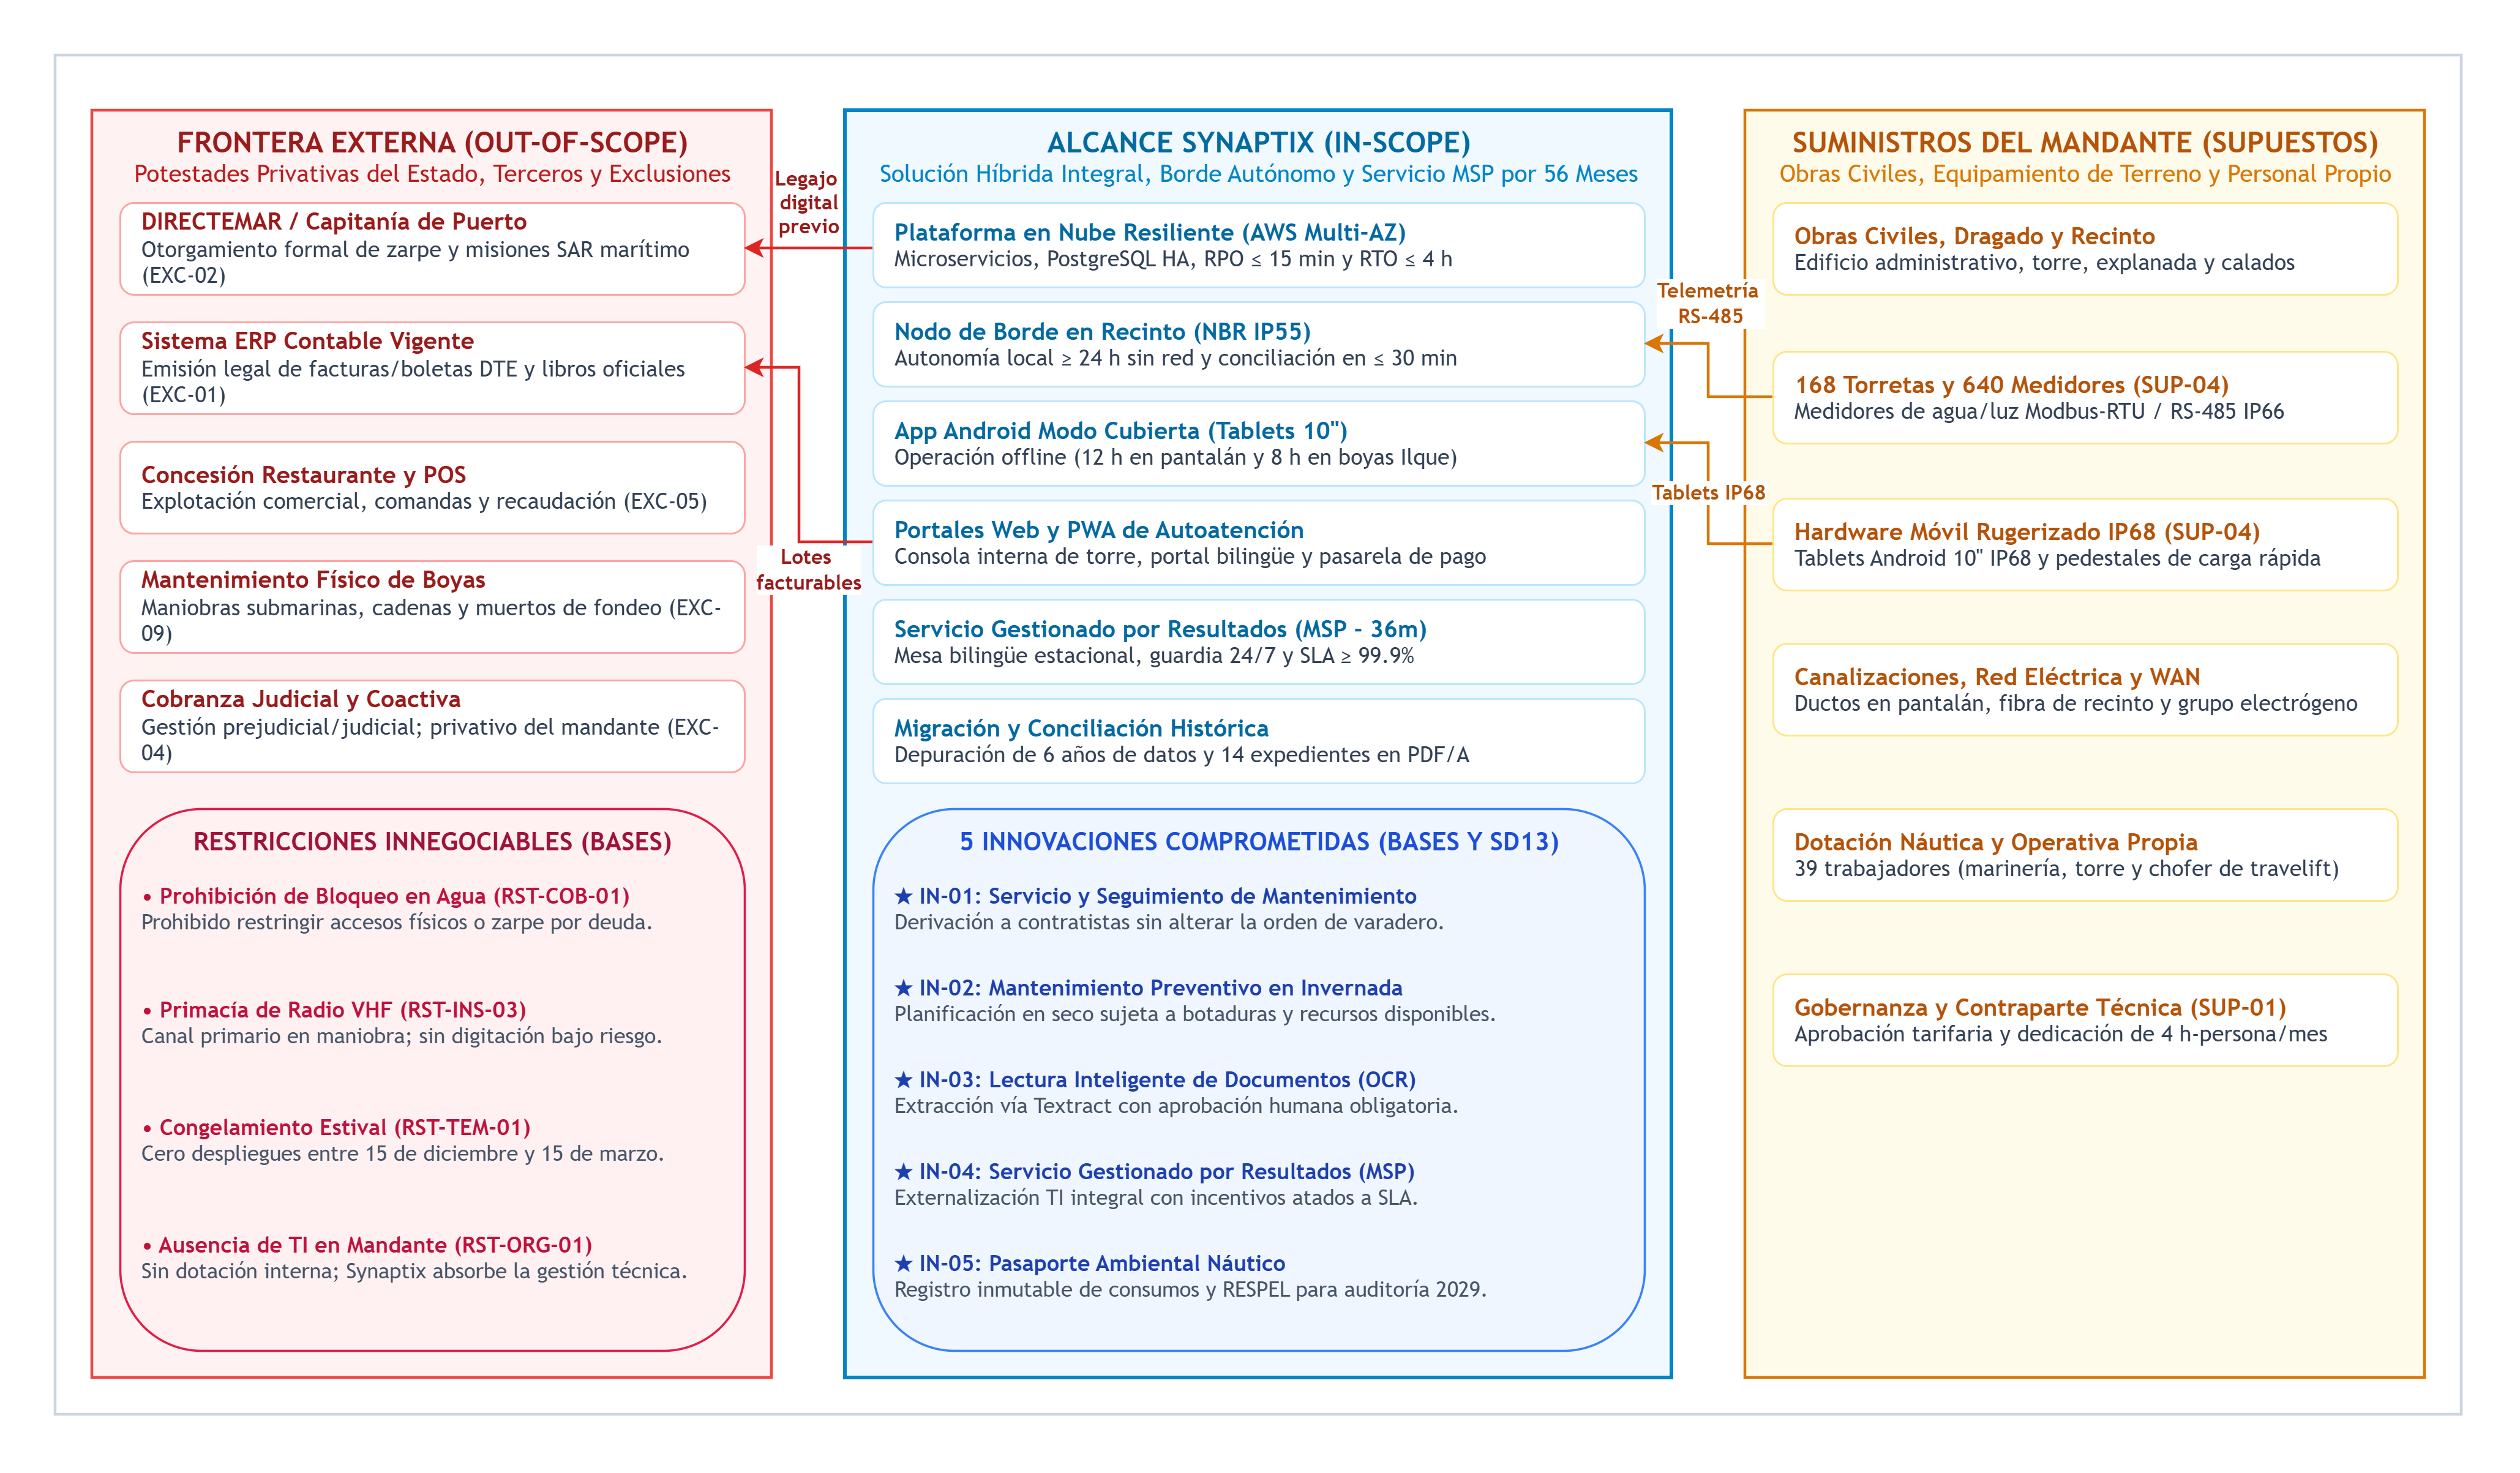
\includegraphics[width=\textwidth]{figuras/diagrama-frontera-alcance.png}
    \caption{Frontera de alcance, suministros del mandante y exclusiones privativas}
    \label{fig:diagrama-frontera-alcance}
    \FuenteTabla{elaboración propia}
\end{figure}

El análisis de los tres pilares de alcance y responsabilidades establece:

\subsubsection{Pilar Central: Alcance Synaptix (IN-SCOPE)}
Synaptix asume el dimensionamiento, la especificación, la configuración, la integración y la verificación del funcionamiento conjunto de la solución. La adquisición del hardware y la ejecución de las obras corresponden al cliente, conforme a EXC-06 y EXC-10. Esta distribución separa compra y construcción de la responsabilidad técnica por el sistema integrado \parencite[cap.~11]{caso07}.
Esto se puede ver a mayor detalle:
\begin{itemize}
    \item \textbf{Plataforma en Nube Resiliente:} Despliegue en AWS Local Zone Santiago bajo esquema multi-AZ, microservicios contenerizados y base de datos relacional PostgreSQL con respaldos cruzados diarios (RTO $\le 4$\,h, RPO $\le 15$\,min).
    \item \textbf{Nodo de Borde en Recinto (NBR):} El NBR se instala en un gabinete mural industrial IP55 en administración y concentra el componente local mínimo para la operación autoadministrada del recinto. La verificación de instalación comprende montaje, alimentación, condiciones térmicas y continuidad operacional. El componente mantiene 24 horas de operación sin enlace WAN y sincroniza automáticamente los registros en $\le 30$ minutos tras la reconexión; estas capacidades responden a la continuidad exigida y a la ausencia de personal TI del cliente \parencite[cap.~15, RT-03.10, RT-03.13 y RT-06.01]{caso07}.
    \item \textbf{Aplicación Móvil Android 10'' (Modo Cubierta):} Diseñada para marinería, escuela de vela y varadero, con autonomía offline de 12 horas en pantalanes y 8 horas en inspección de boyas en Bahía Ilque.
    \item \textbf{Portales Web y PWA de Autoatención:} Consola de operaciones para torre de control y portal de autogestión de socios y visitantes bilingüe (español e inglés), con pasarela de pagos integrada.
    \item \textbf{Servicio Gestionado (MSP) por 36 Meses:} Mesa de ayuda estacional (L1/L2), guardia crítica 24/7/365 para incidentes P1/P2, observabilidad, mantención preventiva y correctiva, y cumplimiento de la disponibilidad mensual de la transacción crítica de extremo a extremo ($\ge 99,9\,\%$), diferenciada de la disponibilidad mensual de los componentes exigidos por la sección 7.2 de las Bases Técnicas Transversales ($\ge 99,95\,\%$). Esta separación permite verificar el servicio recibido por el usuario sin confundirlo con la disponibilidad individual de la infraestructura.
    \item \textbf{Cinco Innovaciones Contractuales:} Incorporación de IN-01 a IN-05 desarrolladas en SD13 y reguladas bajo el Formulario T-19.
\end{itemize}

\subsubsection{Pilar Derecho: Suministros del Mandante (Supuestos y Compras)}
El cliente adquiere el hardware y ejecuta las obras de EXC-06 y EXC-10 a partir de la especificación técnica, el dimensionamiento y los requisitos de recepción entregados por el proponente. Cada adquisición y habilitación se vincula en el cronograma con la instalación y las pruebas dependientes, conforme a SUP-04. Su valorización pertenece a la Oferta Económica; los siguientes ítems establecen los suministros y condiciones técnicas de entrega \parencite[cap.~11]{caso07}.
Bajo esto, al cliente le corresponde:
\begin{itemize}
    \item \textbf{Obras de Habilitación:} Las canalizaciones, obras eléctricas, adecuaciones de torretas y postación permiten instalar los componentes de la solución y son ejecutadas por el cliente. La documentación de entrega comprende planos, cantidades, características y requisitos de recepción; la verificación de integración comprueba su compatibilidad con el equipamiento y las condiciones de pantalán flotante. El alcance corresponde a la habilitación del sistema, no a la mantención general de la infraestructura marítima \parencite[caps.~10--11]{caso07}.
    \item \textbf{Redes Físicas y Respaldo de Energía:} La solución utiliza ductos protegidos para el cableado de pantalán, enlaces de fibra óptica de recinto y respaldo mediante grupo electrógeno automático. Los ductos resguardan el tendido sometido a flexión y humedad; la fibra enlaza los puntos operacionales; y el respaldo de energía sostiene los componentes locales de continuidad. El cliente ejecuta las obras y adquiere los equipos especificados. Las pruebas de aceptación comprueban cobertura, segregación, alimentación y recuperación del servicio \parencite[cap.~10; cap.~15, RT-03.10 y RT-03.24]{caso07}.
    \item \textbf{Submedición y Adecuación de Torretas:} La solución integra 640 medidores: uno de agua y uno de energía por cada amarra, $320 \times 2 = 640$. La comunicación utiliza Modbus-RTU / RS-485 y equipos IP66 para la instrumentación instalada en pantalán, aprovechando la infraestructura de las 168 torretas existentes. La instalación comprende inspección de montaje, cableado y compatibilidad, especificación de adecuaciones y comprobación de cada lectura e imputación. El cliente adquiere los equipos y ejecuta las obras especificadas. El registro de asociación y el informe de puesta en servicio documentan el resultado; la aptitud para ambiente marino se acredita mediante documentación del equipamiento y verificaciones de instalación \parencite[sec.~2.3; caps.~10--11; sec.~14.1]{caso07}.
    \item \textbf{Dispositivos de Terreno:} Los perfiles operacionales utilizan tablets Android de 10'' rugerizadas IP68 y medios de recarga. Su especificación considera lluvia, humedad y trabajo con guantes; las pruebas comprueban legibilidad, interacción, autonomía y conservación de registros fuera de cobertura. El cliente adquiere dispositivos y accesorios conforme a la especificación por perfil, que individualiza cantidad, modelo de referencia, accesorios, gestión, reposición y procedimiento de aceptación. La configuración e integración forman parte de la prestación técnica \parencite[cap.~15, RT-03.10 y RT-12.11]{caso07}.
    \item \textbf{Dotación Operativa Propia:} Disponibilidad de los 39 trabajadores en régimen de invierno (marineros, personal de torre, operarios de cunas y chofer calificado de travelift).
    \item \textbf{Gobernanza y Contraparte Técnica:} El cliente designa la Contraparte Técnica para coordinar la revisión de entregables y pruebas y suscribir las actas de aceptación que le corresponden. Los responsables de procesos aprueban tarifas, reglas comerciales y medidas de cobranza conforme a sus atribuciones. La participación en revisiones, actas y decisiones se registra separadamente de la administración técnica y funcional prestada por el adjudicatario, mediante el método de dimensionamiento vinculado a EST-18.
\end{itemize}

\subsubsection{Pilar Izquierdo: Frontera Externa, Exclusiones y Restricciones (OUT-OF-SCOPE)}
Conforme al capítulo 11 del Caso 07 y a las restricciones innegociables del proyecto:
\begin{itemize}
    \item \textbf{DIRECTEMAR / Capitanía de Puerto (EXC-02, RST-INS-01):} El otorgamiento formal de zarpe es potestad administrativa exclusiva e indelegable de la Autoridad Marítima. Synaptix prepara, valida y custodia el legajo digital previo, pero jamás usurpa la autorización legal del zarpe. Las operaciones de Búsqueda y Salvamento Marítimo (SAR) corresponden privativamente a las Fuerzas Armadas.
    \item \textbf{Sistema ERP Contable Vigente (EXC-01, RST-INS-02):} La emisión de facturas y boletas electrónicas timbradas (DTE) y los libros oficiales tributarios permanecen bajo la competencia exclusiva del software contable del cliente. Synaptix liquida y exporta lotes de hechos facturables conciliados.
    \item \textbf{Concesión y Punto de Venta del Restaurante (EXC-05):} La administración del restaurante y de su punto de venta queda fuera del alcance. La plataforma registra su relación contractual con la marina y los consumos de servicios asociados, sin gestionar comandas ni la operación gastronómica \parencite[cap.~11]{caso07}.
    \item \textbf{Mantenimiento Físico de Boyas y Fondeos (EXC-09):} El mantenimiento de boyas y trenes de fondeo queda fuera de la prestación de Synaptix. La plataforma registra su estado, su ocupación y el cumplimiento del programa de inspección, incluidas las inspecciones desconectadas y los antecedentes de las actuaciones de mantenimiento, sin ejecutar las maniobras físicas.
    \item \textbf{Restricciones Operacionales Innegociables:}
    \begin{enumerate}[label=(\alph*)]
        \item \emph{Restricción de Acceso por Cobranza (RST-COB-01):} Una medida de cobranza que impida el acceso de un armador a su embarcación requiere decisión formal de la compañía, registrada y fundamentada. El sistema conserva la autoridad que la emite, su alcance y evidencia antes de aplicar la medida; la mora no genera por sí sola una restricción automática. La operación de la cobranza judicial y del procedimiento sobre embarcaciones abandonadas queda fuera de la prestación, manteniéndose el expediente trazable requerido (EXC-04) \parencite[caps.~10--11]{caso07}.   
        \item \emph{Uso de Radio VHF (RST-INS-03):} La comunicación VHF continúa como medio primario durante maniobras de atraque e izaje; el sistema no impone digitación manual en momentos de riesgo físico.
    \end{enumerate}
    \item \textbf{Delimitación Geográfica:} La cobertura abarca la dársena principal, los cinco pantalanes de atraque, muelle de espera, explanada de varadero, bodega RESPEL, surtidor de combustible y el campo de boyas exterior en Bahía Ilque (a 6 millas náuticas).
\end{itemize}

\subsection{Catálogo de Requerimientos y Cobertura}

La propuesta comprende 146 requerimientos funcionales (RF) y 56 requerimientos no funcionales (RNF), originados en el Subdocumento 2 (A2.1 y A2.2). Complementariamente, las Bases Técnicas Transversales incorporan 374 requisitos técnicos (RT) codificados en sus capítulos 2 al 26. Los 576 requisitos se individualizan en el \textbf{Formulario T-12}, que registra 146 RF y 56 RNF con declaración SÍ, y 344 RT con declaración SÍ y 30 RT con declaración NO. Estas declaraciones expresan los compromisos y límites de la oferta; su cumplimiento se comprobará mediante los entregables, pruebas y evidencias de aceptación. Las respuestas NO incluyen su justificación, sin que esta constituya por sí sola una exención de los requisitos obligatorios.

La Tabla~\ref{tab:sintesis_requerimientos} desglosa los 146 requerimientos funcionales organizados por grupo modular y nivel de prioridad técnica.

\begin{table}[H]
\centering
\small
\begin{tabularx}{\linewidth}{|X|r|r|r|r|}
\hline
\EncabezadoTabla{Grupo funcional / código} & \EncabezadoTabla{Total RF} & \EncabezadoTabla{Alta} & \EncabezadoTabla{Media} & \EncabezadoTabla{Baja cond.} \\
\hline
Navegación y zarpe (NAV) & 13 & 13 & 0 & 0 \\ \hline
Alertas y comunicaciones (ALE) & 12 & 12 & 0 & 0 \\ \hline
Escuela de vela (ESC) & 14 & 14 & 0 & 0 \\ \hline
Amarras y visitantes (AMA) & 12 & 12 & 0 & 0 \\ \hline
Varadero (VAR) & 8 & 8 & 0 & 0 \\ \hline
Contratistas y portería (CTR) & 7 & 7 & 0 & 0 \\ \hline
Gestión ambiental (AMB) & 7 & 7 & 0 & 0 \\ \hline
Consumos y combustible (CON) & 9 & 8 & 1 & 0 \\ \hline
Boyas y fondeos (BOY) & 7 & 6 & 0 & 1 \\ \hline
Hechos facturables (FAC) & 9 & 9 & 0 & 0 \\ \hline
Administración y datos (ADM) & 37 & 29 & 8 & 0 \\ \hline
Portales y autoatención (AUT) & 11 & 2 & 9 & 0 \\ \hline
\hline
\textbf{Total} & \textbf{146} & \textbf{127} & \textbf{18} & \textbf{1} \\ \hline
\end{tabularx}
\caption{Conteo de requerimientos funcionales por grupo y prioridad}
\label{tab:sintesis_requerimientos}
\FuenteTabla{elaboración propia}
\end{table}

Del universo funcional, 127 requerimientos revisten prioridad Alta por constituir el núcleo irrenunciable de operación, seguridad y soporte normativo. Los 18 de prioridad Media corresponden a facilidades de autoatención y reportes gerenciales complementarios, mientras que el único requerimiento de Baja condicionada corresponde al piloto sensórico exterior RF-BOY-04 en Bahía Ilque, cuya activación queda supeditada a factibilidad técnica de comunicaciones y reposición física (DEC-19).

Por su parte, los 56 RNF establecen las condiciones del estándar operacional de la plataforma en escenarios reales:
\begin{itemize}
    \item \textbf{Rendimiento y Experiencia de Usuario:} Tiempos de respuesta evaluados estrictamente en el percentil 95 (P95) de la interacción del usuario final.
    \item \textbf{Disponibilidad y Confiabilidad:} Disponibilidad mensual de componentes de plataforma $\ge 99,95\,\%$, y disponibilidad transaccional de extremo a extremo $\ge 99,9\,\%$.
    \item \textbf{Resiliencia y Operación Desconectada:} Autonomía operativa de 24 horas sin enlace exterior en el NBR, 12 horas continuas fuera de cobertura en los dispositivos de terreno de pantalán, varadero y escuela, y 8 horas en inspecciones de boyas. Las pruebas de continuidad verificarán estas duraciones sin pérdida de los registros exigidos.
\end{itemize}

La Tabla~\ref{tab:cumplimiento-rt} resume el cumplimiento declarado
de los 374 requisitos técnicos transversales en el Formulario T-12.
Se identifican 344 requisitos con respuesta \textbf{Sí} y 30 con
respuesta \textbf{No}. Los códigos declarados como no cumplidos se
individualizan por grupo; los restantes requisitos de cada grupo
se encuentran declarados como cumplidos. Las justificaciones y
referencias de trazabilidad se presentan en el Formulario T-12.

\begin{longtable}{@{}L{.32\textwidth}
                    L{.08\textwidth}
                    L{.08\textwidth}
                    L{.08\textwidth}
                    L{.34\textwidth}@{}}
    \caption{Cumplimiento declarado de requisitos transversales
    en el Formulario T-12}
    \label{tab:cumplimiento-rt} \\
    \hline
    \EncabezadoTabla{Materia técnica / capítulos} &
    \EncabezadoTabla{Total RT} &
    \EncabezadoTabla{Sí} &
    \EncabezadoTabla{No} &
    \EncabezadoTabla{RT declarados No} \\
    \hline
    \endfirsthead

    \hline
    \EncabezadoTabla{Materia técnica / capítulos} &
    \EncabezadoTabla{Total RT} &
    \EncabezadoTabla{Sí} &
    \EncabezadoTabla{No} &
    \EncabezadoTabla{RT declarados No} \\
    \hline
    \endhead

    Arquitectura híbrida (2 y 3) &
    38 & 34 & 4 &
    RT-02.14; RT-03.08; RT-03.09; RT-03.19. \\
    \hline

    Entrega continua y datos (4 y 5) &
    44 & 41 & 3 &
    RT-04.14; RT-05.24; RT-05.30. \\
    \hline

    Sitios, recuperación y equipos (6, 7 y 8) &
    67 & 62 & 5 &
    RT-06.12; RT-06.15; RT-06.34;
    RT-08.15; RT-08.19. \\
    \hline

    Desempeño, continuidad y seguridad (9, 10 y 11) &
    47 & 45 & 2 &
    RT-09.10; RT-11.21. \\
    \hline

    Identidad y observabilidad (12 y 14) &
    22 & 21 & 1 &
    RT-14.09. \\
    \hline

    Usabilidad, módulos y canales (13, 16 y 17) &
    54 & 51 & 3 &
    RT-16.05; RT-16.26; RT-17.08. \\
    \hline

    Sostenibilidad, IA e innovaciones (15, 18 y 26) &
    27 & 23 & 4 &
    RT-15.05; RT-15.06; RT-18.10; RT-26.08 \\
    \hline

    Gobierno, implantación y servicio (19, 20, 21 y 22) &
    49 & 47 & 2 &
    RT-21.12; RT-22.09. \\
    \hline

    Presencia, video y prototipo (23, 24 y 25) &
    26 & 20 & 6 &
    RT-23.07; RT-23.08; RT-23.09; RT-23.10;
    RT-24.03; RT-25.10. \\
    \hline

    \textbf{Total} &
    \textbf{374} &
    \textbf{344} &
    \textbf{30} &
    \textbf{Detalle y justificaciones en el Formulario T-12.} \\
    \hline
\end{longtable}
\FuenteTabla{elaboración propia}

La cobertura declarada se concentra en los ámbitos de desempeño,
continuidad y seguridad, con 45 de 47 requisitos cumplidos; identidad
y observabilidad, con 21 de 22; y gobierno, implantación y servicio,
con 47 de 49. Estos resultados reflejan el énfasis de la propuesta
en sostener la operación de la marina, controlar los accesos y
establecer condiciones de implementación y soporte.

La mayor proporción de respuestas negativas corresponde al grupo
de presencia, video y prototipo, con 6 de 26 requisitos. En términos
absolutos, también destacan sitios, recuperación y equipos, con
5 requisitos no cumplidos, y arquitectura híbrida, con 4. Las
justificaciones particulares de estas respuestas se encuentran
individualizadas en el Formulario T-12.

Los porcentajes expresan la cobertura declarada de la oferta y
no sustituyen la verificación técnica ni los criterios de aceptación.
Cada respuesta negativa debe evaluarse según la obligatoriedad
y aplicabilidad del requisito; su justificación no constituye por
sí sola una exención contractual. Asimismo, los requisitos declarados
como cumplidos deberán acreditarse mediante los entregables,
pruebas y evidencias previstos en la propuesta.

\subsection{Criterios de Aceptación del Caso}

La recepción de cada entregable comprende su verificación técnica y su aceptación formal por la Contraparte Técnica del mandante, conforme a los Artículos 17 y 18 de las Bases Administrativas y al Formulario T-17. Synaptix ejecuta las pruebas y entrega el artefacto, la evidencia objetiva y reproducible de verificación, la trazabilidad hacia los requerimientos satisfechos y el registro de observaciones resueltas. La Contraparte Técnica revisa el expediente y suscribe el acta correspondiente.

Para que los resultados sean comparables y auditables, cada medición identificará el período, la población evaluada, la fuente, la unidad de medida y el procedimiento de cálculo. Se distinguirán los umbrales establecidos en las bases y el caso de las metas adicionales comprometidas en esta oferta. Los tiempos de las transacciones operacionales críticas se verificarán en el percentil 95 de la experiencia real del usuario; los límites máximos específicos de envío de notificaciones y generación de alertas se comprobarán separadamente.

El procedimiento considera diez días hábiles para la revisión del cliente y diez días hábiles para subsanar las observaciones, conforme al Artículo 18.3. La aceptación de un entregable no extingue la responsabilidad por defectos posteriores ni convalida incumplimientos detectados después de su recepción.

\subsubsection{Compuertas Técnicas de Calidad (Quality Gates)}
El cierre de cada marcha blanca y el paso a producción requieren el cumplimiento copulativo de las seis condiciones del Artículo 17.3 de las Bases Administrativas:
\begin{enumerate}
    \item \textbf{Incidentes:} ausencia de incidentes abiertos de severidad crítica o alta atribuibles a la solución, acreditada mediante el registro de incidentes y sus evidencias de resolución.

    \item \textbf{Operación real:} cumplimiento del volumen de operación comprometido en el plan de implantación durante, al menos, las cuatro últimas semanas del período, demostrado mediante registros de transacciones y operaciones efectivamente realizadas.

    \item \textbf{Disponibilidad y respuesta:} cumplimiento sostenido de los indicadores comprometidos durante esas mismas cuatro semanas, respaldado por registros de observabilidad y mediciones de la experiencia real del usuario.

    \item \textbf{Conciliación:} ausencia de diferencias no explicadas entre la solución y el sistema o registro vigente, acreditada mediante recuentos, sumas de control, cruces y documentación de las diferencias identificadas.

    \item \textbf{Capacitación:} personal del cliente capacitado y certificado conforme al plan aprobado, con registros de participación y resultados de las evaluaciones.

    \item \textbf{Aceptación formal:} acta correspondiente suscrita por la Contraparte Técnica.
\end{enumerate}

Las pruebas de reversión en Preproducción y de continuidad desconectada complementan estas condiciones para verificar la recuperación operacional y la conservación de los datos. La continuidad se comprobará durante 24 horas sin enlace exterior en el NBR, 12 horas continuas fuera de cobertura en los dispositivos de pantalán, varadero y escuela, y 8 horas en inspección de boyas, sin pérdida de los registros exigidos. Tras la reconexión del recinto, la sincronización automática no superará 30 minutos.

Si alguna condición de cierre no se cumple, la marcha blanca se extenderá a costo del adjudicatario, sin cargo adicional al cliente ni desplazamiento de las fechas contractuales de las fases siguientes, y con aplicación de las disposiciones sobre atraso del Artículo 80. La fecha programada, la finalización de las pruebas o la entrega de un informe no sustituyen el acta de aceptación.

\subsubsection{Compromiso Detallado con los 25 Criterios de Aceptación (CA-01 a CA-25)}
Los criterios siguientes identifican su recepción por etapa, el método de verificación y la evidencia correspondiente. Su agrupación distingue las capacidades recibidas en cada compuerta de los resultados que requieren seguimiento durante la operación. Las metas adicionales de la oferta se diferencian expresamente de los límites establecidos por el caso. La aceptación formal corresponde a la Contraparte Técnica conforme al procedimiento anterior.

\begin{enumerate}
    \item \textbf{Operación Náutica y Tráfico de Amarras --- Gate 1:}
    \begin{itemize}
        \item \emph{CA-01 (Estado de Amarras):} Estado operacional consultable de las 320 amarras, con identificación de la embarcación presente o salida y actualización del indicador analítico de ocupación en $\le 60$ segundos desde el evento. Se contrastarán los registros con rondas físicas de marinería. La exactitud $\ge 98\,\%$ constituye una meta adicional de la oferta; el informe conservará las discrepancias y sus correcciones.

        \item \emph{CA-02 (Regreso y Plan Vencido):} Registro de salida y regreso en $\le 10$ segundos y un máximo de dos interacciones; alerta visible para la guardia en $\le 15$ minutos desde el vencimiento de un plan sin cierre. Se probarán por separado el registro del regreso, el cierre del plan y la alerta, conservando sus marcas de tiempo.

        \item \emph{CA-03 (Planes Voluntarios):} Creación, cierre y puesta a disposición del plan para las personas autorizadas, con consentimiento explícito y revocable. La recepción funcional verificará permisos y trazabilidad del ciclo completo. Separadamente, el seguimiento de adopción medirá las metas adicionales de 50\,\% al mes 16 y 80\,\% al mes 21 sobre armadores con contrato activo, manteniendo el carácter voluntario del plan.

        \item \emph{CA-08 (Compatibilidad Física y Correspondencia Tarifaria):} Verificación separada de las dimensiones y restricciones físicas de la amarra, y de la correspondencia entre embarcación, tramo contratado y tarifa pagada. El cruce de ocupación y contratos deberá alcanzar cero amarras ocupadas por una eslora que no corresponde al tramo contratado, frente al 22\,\% del caso. Las pruebas de asignación rechazarán puestos físicamente incompatibles y conservarán la matriz de compatibilidad y los resultados del cruce.

        \item \emph{CA-10 (Atención a Visitas):} Asignación y confirmación de amarra compatible en $\le 45$ segundos desde la consulta por radio. Se medirá la transacción completa en terreno, conservando los tiempos y el resultado de compatibilidad.

        \item \emph{CA-13 (Legajo de Zarpe):} Conformación de nómina y antecedentes en $\le 90$ segundos, con comprobación de vigencia documental. El informe conservará el legajo y los tiempos. Como meta adicional, las correcciones manuales se reducirán a $\le 5\,\%$, respecto del 34\,\% registrado en el caso.
    \end{itemize}

    \item \textbf{Seguridad y Escuela de Vela --- Gate 1:}
    \begin{itemize}
        \item \emph{CA-04 (Marejada):} Notificación de emergencia a los 296 armadores mediante SMS, mensajería instantánea y correo electrónico de forma simultánea. Para incluir el tiempo completo de preparación y despacho, la medición operacional comienza con la recepción del aviso oficial en torre y termina con el último envío, sin superar diez minutos. El registro de campaña acreditará destinatario, canal, hora de envío y acuse disponible, con escalamiento telefónico trazable a quienes no acusen recibo. El envío y el acuse se medirán separadamente.

        \item \emph{CA-05 (Contactos):} Detección y actualización trazable de datos obsoletos. Como meta adicional, los contratos activos con contactos obsoletos se reducirán a $\le 5\,\%$, frente al 47\,\% del caso. Se verificará mediante revisión del padrón y evidencias de actualización.

        \item \emph{CA-06 (Salida Escolar):} Registro de una clase de hasta 18 embarcaciones en $\le 60$ segundos, identificando autorización, alumno, bote, monitor, salida y regreso. La consulta de quién permanece en el agua estará disponible en tiempo real. Las pruebas conservarán la nómina y los registros temporales.

        \item \emph{CA-07 (Retiro de Menores):} Registro de solicitud y entrega autorizada, visible inmediatamente para escuela y portería. Se ensayarán el retiro anticipado y el rechazo de una entrega no autorizada, con evidencia de permisos y sincronización.

        \item \emph{CA-23 (Información a Apoderados):} Consulta y aviso de salida y regreso sin llamadas a la escuela ni filmación de alumnos. El envío del aviso en $\le 5$ minutos constituye una meta adicional. Se verificarán el destinatario autorizado, el evento y las marcas de envío.
    \end{itemize}

    \item \textbf{Gestión Comercial, Varadero y Contratistas --- Gate 2:}
    \begin{itemize}
        \item \emph{CA-09 (Oferta Automática de Vacantes):} La confirmación de una vacante definitiva activa automáticamente la oferta al candidato compatible de la lista de espera, con trazabilidad del orden, oferta y respuesta. Se compromete emitir la oferta en $\le 24$ horas desde la confirmación de la vacante, como meta adicional de atención. La medición termina con la emisión de la oferta, distinguiéndola de la aceptación del candidato y de la adjudicación efectiva. Se comprobará mediante simulación de cola y registro de ofertas.

        \item \emph{CA-11 (Recaladas Facturables):} Cero recaladas facturables omitidas, frente al 9\,\% del caso. El cruce entre torre, estancias y hechos facturables conservará la conciliación y la explicación de las diferencias.

        \item \emph{CA-12 (Reservas de Visitantes):} Registro único de reservas recibidas por todos los canales, con origen e historial de cambios. Se ensayará una reserva por cada canal y se verificará su incorporación al mismo registro operacional.

        \item \emph{CA-14 (Plan Previo de Izaje):} Toda maniobra de travelift contará con plan técnico antes del movimiento de carga. Se verificará mediante el cruce entre maniobras y planes, con versión, embarcación y evidencia de preparación previa.

        \item \emph{CA-15 (Reprogramación):} Las faenas afectadas se suspenden inmediatamente ante el aviso de autoridad y se reprograman considerando sus dependencias. Como meta adicional, el despacho de avisos de la nueva agenda a los armadores afectados se completará en $\le 15$ minutos desde su confirmación. Se conservarán el aviso de autoridad, la agenda confirmada, sus marcas temporales, los destinatarios y los envíos fallidos.

        \item \emph{CA-16 (RESPEL):} Trazabilidad completa desde la embarcación generadora hasta la entrega al gestor autorizado, incluyendo lote, pesaje, manifiesto y precarga de antecedentes para SIDREP. Se comprobará mediante seguimiento de lotes y conciliación de la documentación de entrega.

        \item \emph{CA-17 (Contratistas):} Acreditación de las 62 empresas y verificación de la documentación y capacitación ambiental y de seguridad vigentes del personal habilitado, incluyendo los 140 operarios identificados en el alcance. Las pruebas comprobarán vigencias y rechazo de accesos sin habilitación, conservando el registro de acreditación y su resultado.

        \item \emph{CA-24 (Continuidad del Plan de Izaje):} Operadores antiguos y nuevos utilizarán el mismo registro de puntos y posiciones de eslingas antes del izaje. La evidencia se capturará con la embarcación en calzos, no suspendida, para registrar el conocimiento sin introducir riesgos durante la maniobra. La prueba verificará la recuperación del plan por ambos operadores y la trazabilidad de su versión.
    \end{itemize}

    \item \textbf{Criterios Distribuidos y Evidencia Ambiental:}
    \begin{itemize}
        \item \emph{CA-18 (Consumo por Amarra):} Gate 1 verifica captura y consulta individual de agua y energía en las 320 amarras, mediante los 640 puntos de medición definidos, y actualización al menos horaria. Gate 2 verifica su transformación en hechos facturables y su utilización en el indicador ambiental. Se conservarán lecturas, cruces y conciliación. El porcentaje de costo no recuperado se calculará como $100 \times (C-R)/C$, donde $C$ corresponde al costo pagado al distribuidor y $R$ al importe recuperado de los armadores por los mismos servicios y período. La referencia será $<5\,\%$, frente al 38\,\% del caso. La emisión o imputación de un cargo no se contabilizará por sí sola como recuperación; si $C=0$, el indicador se registrará como no aplicable.

        \item \emph{CA-19 (Cierre Ambiental):} El expediente identificará las tres no conformidades, las acciones ejecutadas y sus evidencias de residuos, medición y formación. La serie ambiental será trazable y se consolidará diariamente. Su suficiencia y el cierre de las tres no conformidades se acreditarán mediante el resultado de auditoría antes de la temporada 2029. La recepción técnica de las funciones en Gate 2 y la retención de series por cinco años son verificaciones distintas de este resultado.

        \item \emph{CA-20 (Boyas):} Gate 1 verifica para las 40 boyas quién ocupa cada una, el estado del tren de fondeo y su última inspección; Gate 2 verifica la continuidad del registro integrado. La prueba combinará consulta operacional, historial y una jornada de inspección con ocho horas sin cobertura, seguida de sincronización.

        \item \emph{CA-21 (Facturación):} Gate 2 verifica el proceso sin cuadernos, su conciliación y el registro de notas de crédito por error. Como metas adicionales, el esfuerzo de preparación se reducirá de diez a dos días-persona mensuales y las notas de crédito por error a menos del 1\,\%. Se medirán el esfuerzo administrativo y la proporción de documentos corregidos en los cierres observados.

        \item \emph{CA-22 (Abandono):} Gate 2 verifica los 14 expedientes completos, digitalizados, indexados y foliados en PDF/A. Se cotejará cada expediente con sus fuentes migradas, conservando el inventario y la trazabilidad probatoria.
    \end{itemize}

    \item \textbf{CA-25 --- Recepción y Seguimiento Transversal:}
    Gate 1 verifica continuidad y operabilidad del alcance de E1; Gate 2 verifica la preparación del servicio integral. Durante los 36 meses de operación, el Gerente de Servicio mantiene la gestión técnica sin requerir personal informático del cliente. La disponibilidad mensual de la transacción crítica de extremo a extremo será $\ge 99,9\,\%$; los componentes sujetos a la sección 7.2 de las Bases Técnicas Transversales cumplirán $\ge 99,95\,\%$. Los informes de disponibilidad, incidentes, mantenimiento y continuidad acreditarán el cumplimiento efectivo durante el servicio, complementando las verificaciones iniciales de recepción.
\end{enumerate}

\newpage
\section{Esquema de solución}

La Figura~\ref{fig:esquema-solucion} organiza la solución en cuatro
ámbitos: actores, interfaces de acceso, servicios funcionales e
integraciones externas. Esta vista presenta la organización conceptual del alcance y permite reconocer quién utiliza la plataforma, mediante qué canales accede y cuáles son las capacidades comprendidas dentro de su frontera.

\begin{figure}[H]
    \centering
    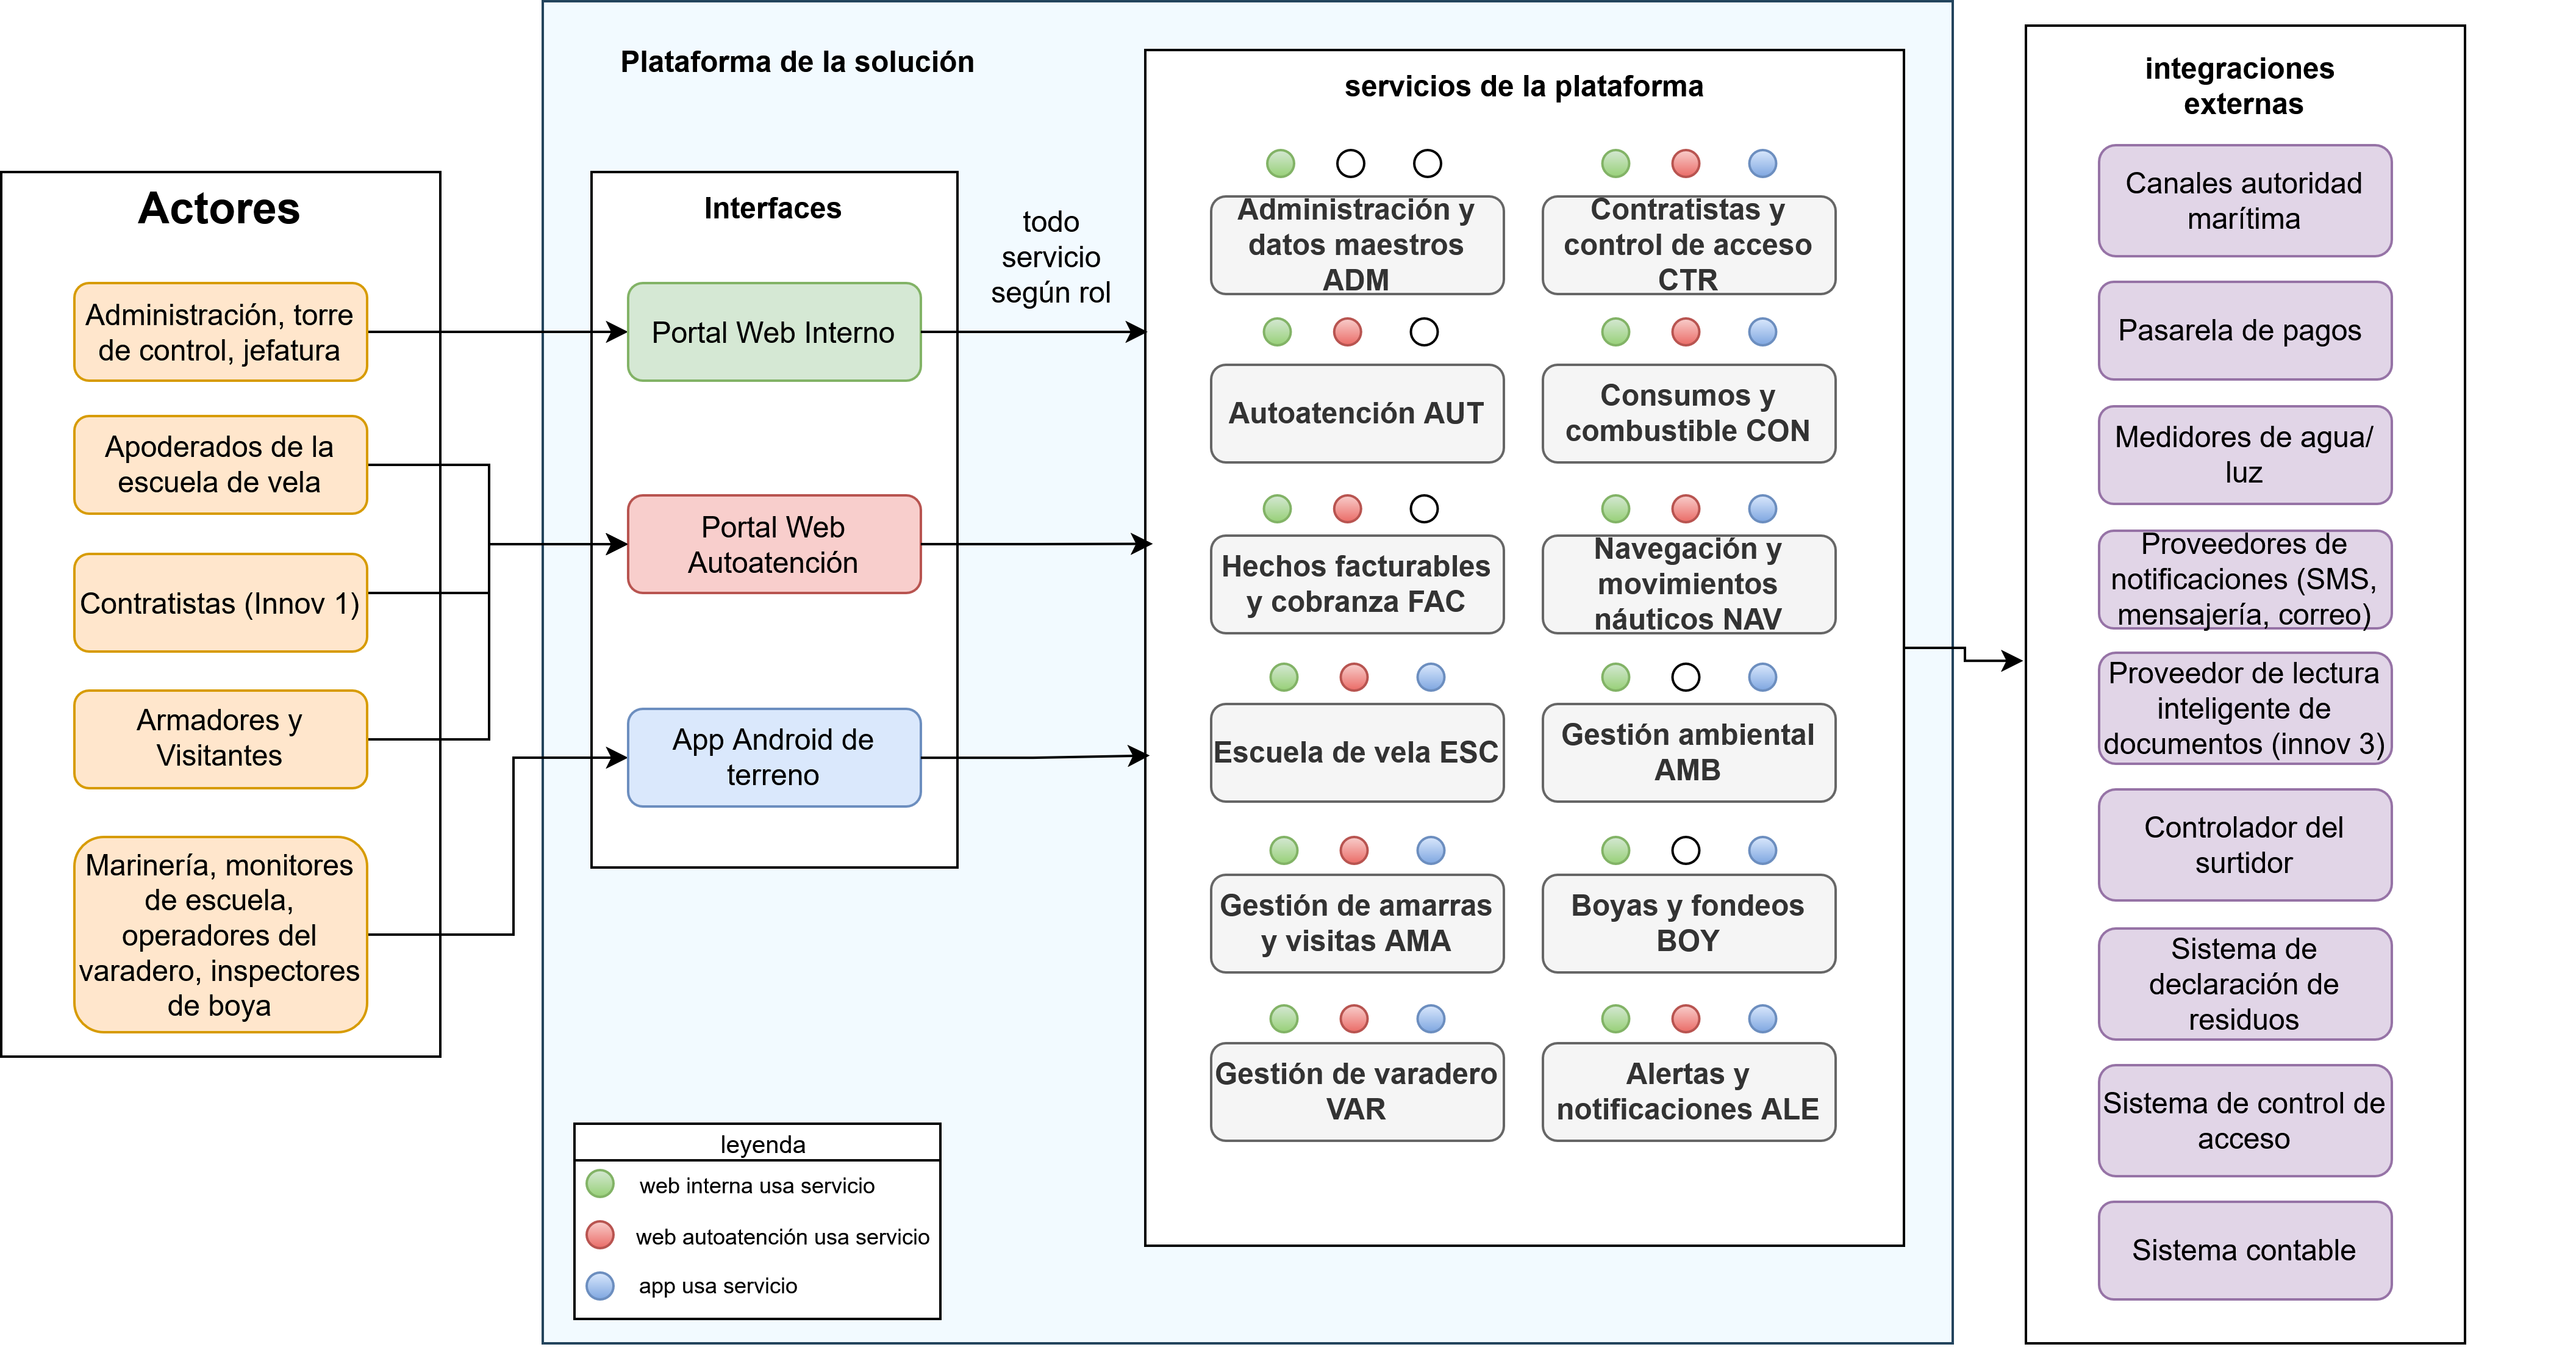
\includegraphics[width=\textwidth]{figuras/esquema-solucion.png}
    \caption{Modelo conceptual de la solución.}
    \label{fig:esquema-solucion}
    \FuenteTabla{elaboración propia}
\end{figure}

Los actores se agrupan según su participación en la marina: administración, torre de control y jefatura; apoderados de la escuela de vela; contratistas vinculados con la innovación 1; armadores y visitantes; y personal de terreno. Su participación se canaliza mediante las interfaces y queda delimitada por el rol de cada usuario.

Las tres interfaces separan las formas de interacción de las funciones que presta la plataforma. El Portal Web Interno atiende las gestiones del personal autorizado; el Portal Web Autoatención permite la interacción de los usuarios externos; y la App Android de terreno proporciona el canal móvil.

Los círculos situados sobre cada servicio permiten identificar qué interfaces lo utilizan: verde para la web interna, rojo para autoatención y azul para la aplicación. Todos los servicios presentan acceso desde la web interna, mientras que la participación de los otros canales varía según la capacidad.

Los doce servicios descomponen el alcance en responsabilidades diferenciadas. NAV, AMA y ESC distinguen la navegación, la gestión de amarras y visitas, y la escuela de vela; VAR, CTR y BOY delimitan las capacidades de varadero, contratistas y control de acceso, y boyas y fondeos. CON, AMB y FAC separan los consumos y combustible, la gestión ambiental y los hechos facturables y cobranza. ADM, AUT y ALE aportan capacidades compartidas de administración, autoatención y comunicaciones. Esta separación permite reconocer qué ámbito atiende cada necesidad sin convertir el esquema en un catálogo detallado de requerimientos.

En particular, el Portal Web Autoatención y AUT no representan la misma pieza: el primero es una interfaz de acceso y el segundo es el servicio funcional que canaliza las interacciones hacia las capacidades responsables. Asimismo, ADM reúne la administración y los datos maestros, mientras que ALE atiende las alertas y notificaciones de distintos ámbitos de la solución.

El contenedor central establece la frontera de la plataforma. Los nueve elementos situados a su derecha corresponden a integraciones externas: canales de la autoridad marítima, pasarela de pagos, medidores de agua y luz, proveedores de notificaciones y lectura inteligente de documentos, controlador del surtidor y sistemas de declaración de residuos, control de acceso y contabilidad. Su ubicación diferencia las funciones propias de la plataforma de los equipos y servicios con los que debe relacionarse. La conexión conjunta expresa esa necesidad de integración, sin establecer por sí sola una dirección de intercambio ni una asociación individual con cada módulo. El diagrama de contexto y las descomposiciones posteriores desarrollan esas relaciones con mayor detalle.

La Figura~\ref{fig:diagrama-contexto} desarrolla las relaciones entre actores, unidades funcionales y servicios externos. Identifica las tareas de los participantes y los intercambios que conectan las capacidades de la plataforma, incluidas las solicitudes de mantenimiento de IN-01 y la extracción documental asistida de IN-03.

\begin{figure}[H]
    \centering
    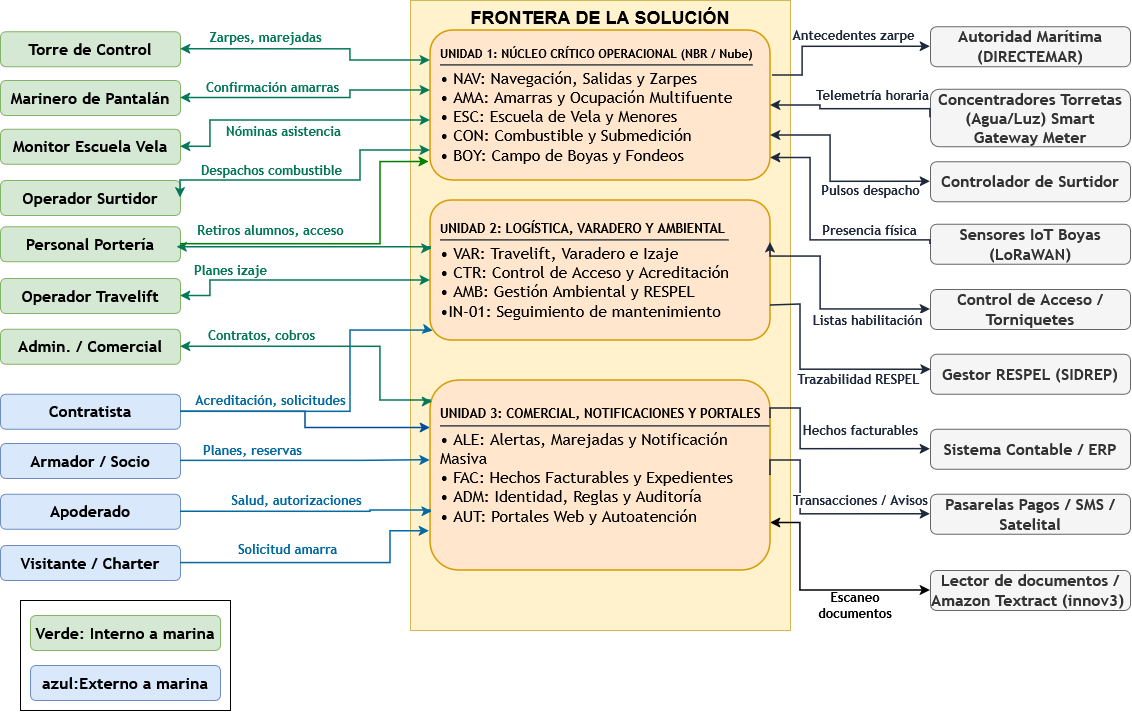
\includegraphics[width=\textwidth]{figuras/diagrama-contexto.png}
    \caption{Diagrama de contexto de la solución}
    \label{fig:diagrama-contexto}
    \FuenteTabla{elaboración propia}
\end{figure}

La Unidad 1 concentra los módulos NAV, AMA, ESC, CON y BOY,
correspondientes a la operación náutica y de terreno. La torre
de control utiliza los antecedentes de navegación y amarras
para coordinar movimientos y preparar el legajo de zarpe;
marinería registra salidas, regresos y verificaciones de ocupación.
Los monitores mantienen la participación y los movimientos
de las clases de vela, mientras que el personal del surtidor
registra los despachos y su evidencia de recepción. BOY conserva
el inventario y las observaciones e inspecciones del campo
de fondeos. La indicación NBR/Nube expresa que las funciones
críticas disponen de ejecución local y posterior conciliación,
según el alcance de continuidad definido para la plataforma.

La Unidad 2 reúne VAR, CTR y AMB para relacionar la programación
del varadero, las condiciones de ejecución de las faenas,
la habilitación de contratistas y la trazabilidad ambiental.
El operador de travelift consulta los planes de izaje y registra
las actuaciones en condiciones seguras. Portería verifica
la identidad y habilitación de las personas que solicitan acceso,
vinculando esa comprobación con la faena autorizada.
Los antecedentes ambientales permiten relacionar los residuos
con la embarcación y el trabajo que los generó, y conservar
las evidencias de su entrega y gestión posterior.

Las restantes innovaciones complementan componentes existentes para evitar procesos paralelos y conservar la trazabilidad de la solución. IN-02 incorpora la coordinación preventiva de invernada sobre VAR, CTR, AUT, ALE y ADM, reutilizando las solicitudes de IN-01 y manteniendo la elección de trabajos y contratista por el armador.

IN-04 incorpora IN4-MET al ámbito de Varadero y contratistas, relacionado con VAR y CTR, e IN4-CON al ámbito de Finanzas y cobranza, relacionado con FAC. AUT ofrece el canal de interacción y ADM administra los permisos. Estos componentes registran el esfuerzo activo y preparan el expediente de reconocimiento variable, sin sustituir el servicio gestionado obligatorio.

IN-05 incorpora planes voluntarios de reducción de agua al ámbito ambiental y de consumos. Utiliza AUT y ADM para la consulta y los permisos, y reutiliza mediciones y permanencias validadas sin modificar los hechos facturables.

La recepción técnica comprueba interfaces, permisos, trazabilidad y continuidad de los procesos base. Los calendarios de incorporación se establecen en el alcance por etapas; los pilotos y protocolos de comprobación del beneficio se desarrollan en las secciones 13.2, 13.4 y 13.5 y en el Formulario T-19.

La Unidad 3 agrupa FAC, ADM, AUT y ALE para atender las gestiones
comerciales, los datos maestros, los permisos y las comunicaciones.
Administración consulta contratos, cuentas y conciliaciones;
los armadores y visitantes presentan planes, reservas y solicitudes;
los apoderados gestionan antecedentes y autorizaciones;
y los contratistas aportan documentación y consultan las actuaciones
habilitadas para su perfil. AUT canaliza estas interacciones
hacia el módulo responsable. ALE gestiona los avisos originados
en las tres unidades, conservando el seguimiento de los envíos
y los resultados disponibles.

Las unidades colaboran mediante los hechos registrados
en cada proceso. Una estadía confirmada, un consumo medido,
un despacho de combustible o una prestación de varadero
pueden originar un hecho facturable que FAC valida y remite
al sistema contable. ADM mantiene los antecedentes y permisos
necesarios para esas actuaciones, mientras que AUT permite
consultar sus resultados. Esta colaboración conserva la relación
entre el registro operacional, su evidencia y su tratamiento
administrativo, evitando que cada área mantenga una versión
independiente del mismo hecho.

Las integraciones de la Unidad 1 aportan antecedentes
para la operación y la medición. Los concentradores de torretas
entregan lecturas identificadas de agua y electricidad,
que CON relaciona con la amarra y el contrato correspondiente.
La instrumentación del surtidor aporta datos para conciliar
los despachos registrados por el operador. Los canales
de la Autoridad Marítima permiten comunicar antecedentes
de zarpe y recibir avisos oficiales por los medios autorizados;
el otorgamiento del zarpe permanece fuera de la responsabilidad
de Synaptix. La integración sensórica de boyas corresponde
a un piloto condicionado a su aprobación y a la acreditación
de alimentación y comunicaciones, sin sustituir las inspecciones
desconectadas.

En el ámbito logístico y ambiental, el control de acceso
existente intercambia habilitaciones y resultados de verificación
con CTR. Las relaciones de gestión de residuos comprenden
dos responsabilidades distintas: la declaración mediante SIDREP,
cuando corresponda, y la recepción y tratamiento material
por gestores autorizados. Synaptix prepara y conserva
los antecedentes y constancias de estas actuaciones,
sin asumir las funciones materiales del gestor.

Las integraciones comerciales y de comunicación complementan
las funciones de la Unidad 3. El sistema contable recibe
hechos facturables y devuelve documentos emitidos, pagos
y resultados de conciliación, manteniendo la emisión tributaria.
Las pasarelas procesan pagos autorizados; los proveedores
de SMS, mensajería y correo transportan notificaciones;
y el canal de baja capacidad permite intercambiar mensajes
con embarcaciones fuera de cobertura convencional.
Cada intercambio conserva su identificador y estado
para distinguir una solicitud enviada de una actuación
efectivamente confirmada.

Finalmente, IN-03, \textit{Lectura inteligente de documentos para el ingreso asistido de antecedentes},
utiliza Amazon Textract para obtener texto y campos propuestos
a partir de documentos digitalizados. La plataforma presenta
esos resultados a la persona autorizada del dominio,
quien los revisa, corrige y aprueba antes de incorporarlos
al registro correspondiente. Se conservan el original,
la salida del procesamiento y la decisión humana.
El ingreso manual permanece disponible ante errores
o indisponibilidad del proveedor, de modo que la asistencia
documental no impida la continuidad de la solución base.


\subsection{Sistemas y entornos externos}

Los intercambios identificados en el diagrama de contexto relacionan la
operación del recinto con servicios, equipos y entidades que permanecen
fuera de la solución. Cada relación se interpreta según los antecedentes
recibidos o entregados, el responsable de la actuación y la evidencia
disponible de su resultado. Las dependencias del Anexo A2.6 del
Subdocumento 2 delimitan las condiciones de integración; su representación
no presupone una interfaz automática disponible ni una actuación ya
ejecutada.

El sistema contable recibe los hechos facturables previamente validados
y devuelve antecedentes de documentos emitidos, pagos y rechazos. Los
servicios de pago aportan el resultado identificado de la transacción,
mientras que los proveedores de comunicación permiten despachar mensajes
y conocer los estados que efectivamente informen. La plataforma conserva
la relación entre solicitud, envío y respuesta. La ausencia de una
respuesta válida permanece como una situación pendiente, sin presentarse
como confirmación del resultado.

Los equipos del recinto aportan lecturas de consumo, antecedentes
meteorológicos y estados de los sistemas existentes de acceso. Su
utilización depende de interfaces disponibles, documentadas y verificadas.
Los registros recibidos conservan origen y momento de captura, de modo
que pueda distinguirse información vigente, observaciones históricas y
datos que requieren revisión. La utilización de estos antecedentes no
sustituye las comprobaciones que corresponden al personal responsable
de cada actuación.

La Autoridad Marítima proporciona avisos oficiales y recibe los
antecedentes exigibles de zarpe mediante los canales admitidos. En la
gestión ambiental, SIDREP corresponde al entorno de declaración de
residuos, mientras que los gestores autorizados realizan las actuaciones
materiales de recepción, transporte o tratamiento y proporcionan sus
certificados. Estas relaciones se mantienen diferenciadas: presentar una
declaración no acredita por sí mismo la entrega física ni la disposición
final del residuo.

\subsection{Descomposición Funcional por Unidades Operacionales}

Marina-Ops, Marina-Log y Marina-Admin agrupan las funciones para explicar la colaboración entre operación náutica, servicios de terreno y gestión administrativa. Los códigos NAV, AMA, ESC, CON, BOY, VAR, CTR, AMB, FAC, ADM, AUT y ALE identifican los grupos del catálogo funcional del Anexo A2.1 del Subdocumento 2. Su correspondencia con los componentes de la arquitectura lógica se mantiene mediante el Formulario T-12.

Las tres vistas siguientes distinguen participantes, funciones e interlocutores. Los participantes aportan antecedentes o realizan actuaciones; los módulos comprueban y conservan resultados; y las conexiones identifican información intercambiada con otras unidades o entidades externas. Un interlocutor situado fuera del contenedor de una unidad puede seguir perteneciendo a la solución. La posición gráfica no determina la dirección del intercambio ni acredita un protocolo de integración.

Las unidades colaboran mediante los hechos registrados en cada proceso. Una estadía, un consumo, un despacho de combustible o una prestación de varadero conservan su origen operacional antes de ser utilizados en el tratamiento comercial. Del mismo modo, una solicitud presentada mediante autoatención se dirige al responsable funcional sin sustituir las comprobaciones necesarias para autorizarla.

ALE aparece en la agrupación administrativa del contexto, pero presta funciones de comunicación a las tres unidades. Los canales de atención, los controles de acceso a la información y la continuidad local también atraviesan esta agrupación. Su tratamiento común se desarrolla después de las vistas particulares, manteniendo la responsabilidad del módulo que origina cada actuación.

\subsection{Marina-Ops: operación náutica y de terreno}

Marina-Ops reúne las funciones que relacionan embarcaciones, puestos,
participantes y registros de terreno.
La Figura~\ref{fig:descomposicion-marina-ops} muestra cómo NAV, AMA,
ESC, CON y BOY producen antecedentes operacionales y los entregan
a otros responsables.

\begin{figure}[H]
    \centering
    \makebox[\textwidth][c]{%
        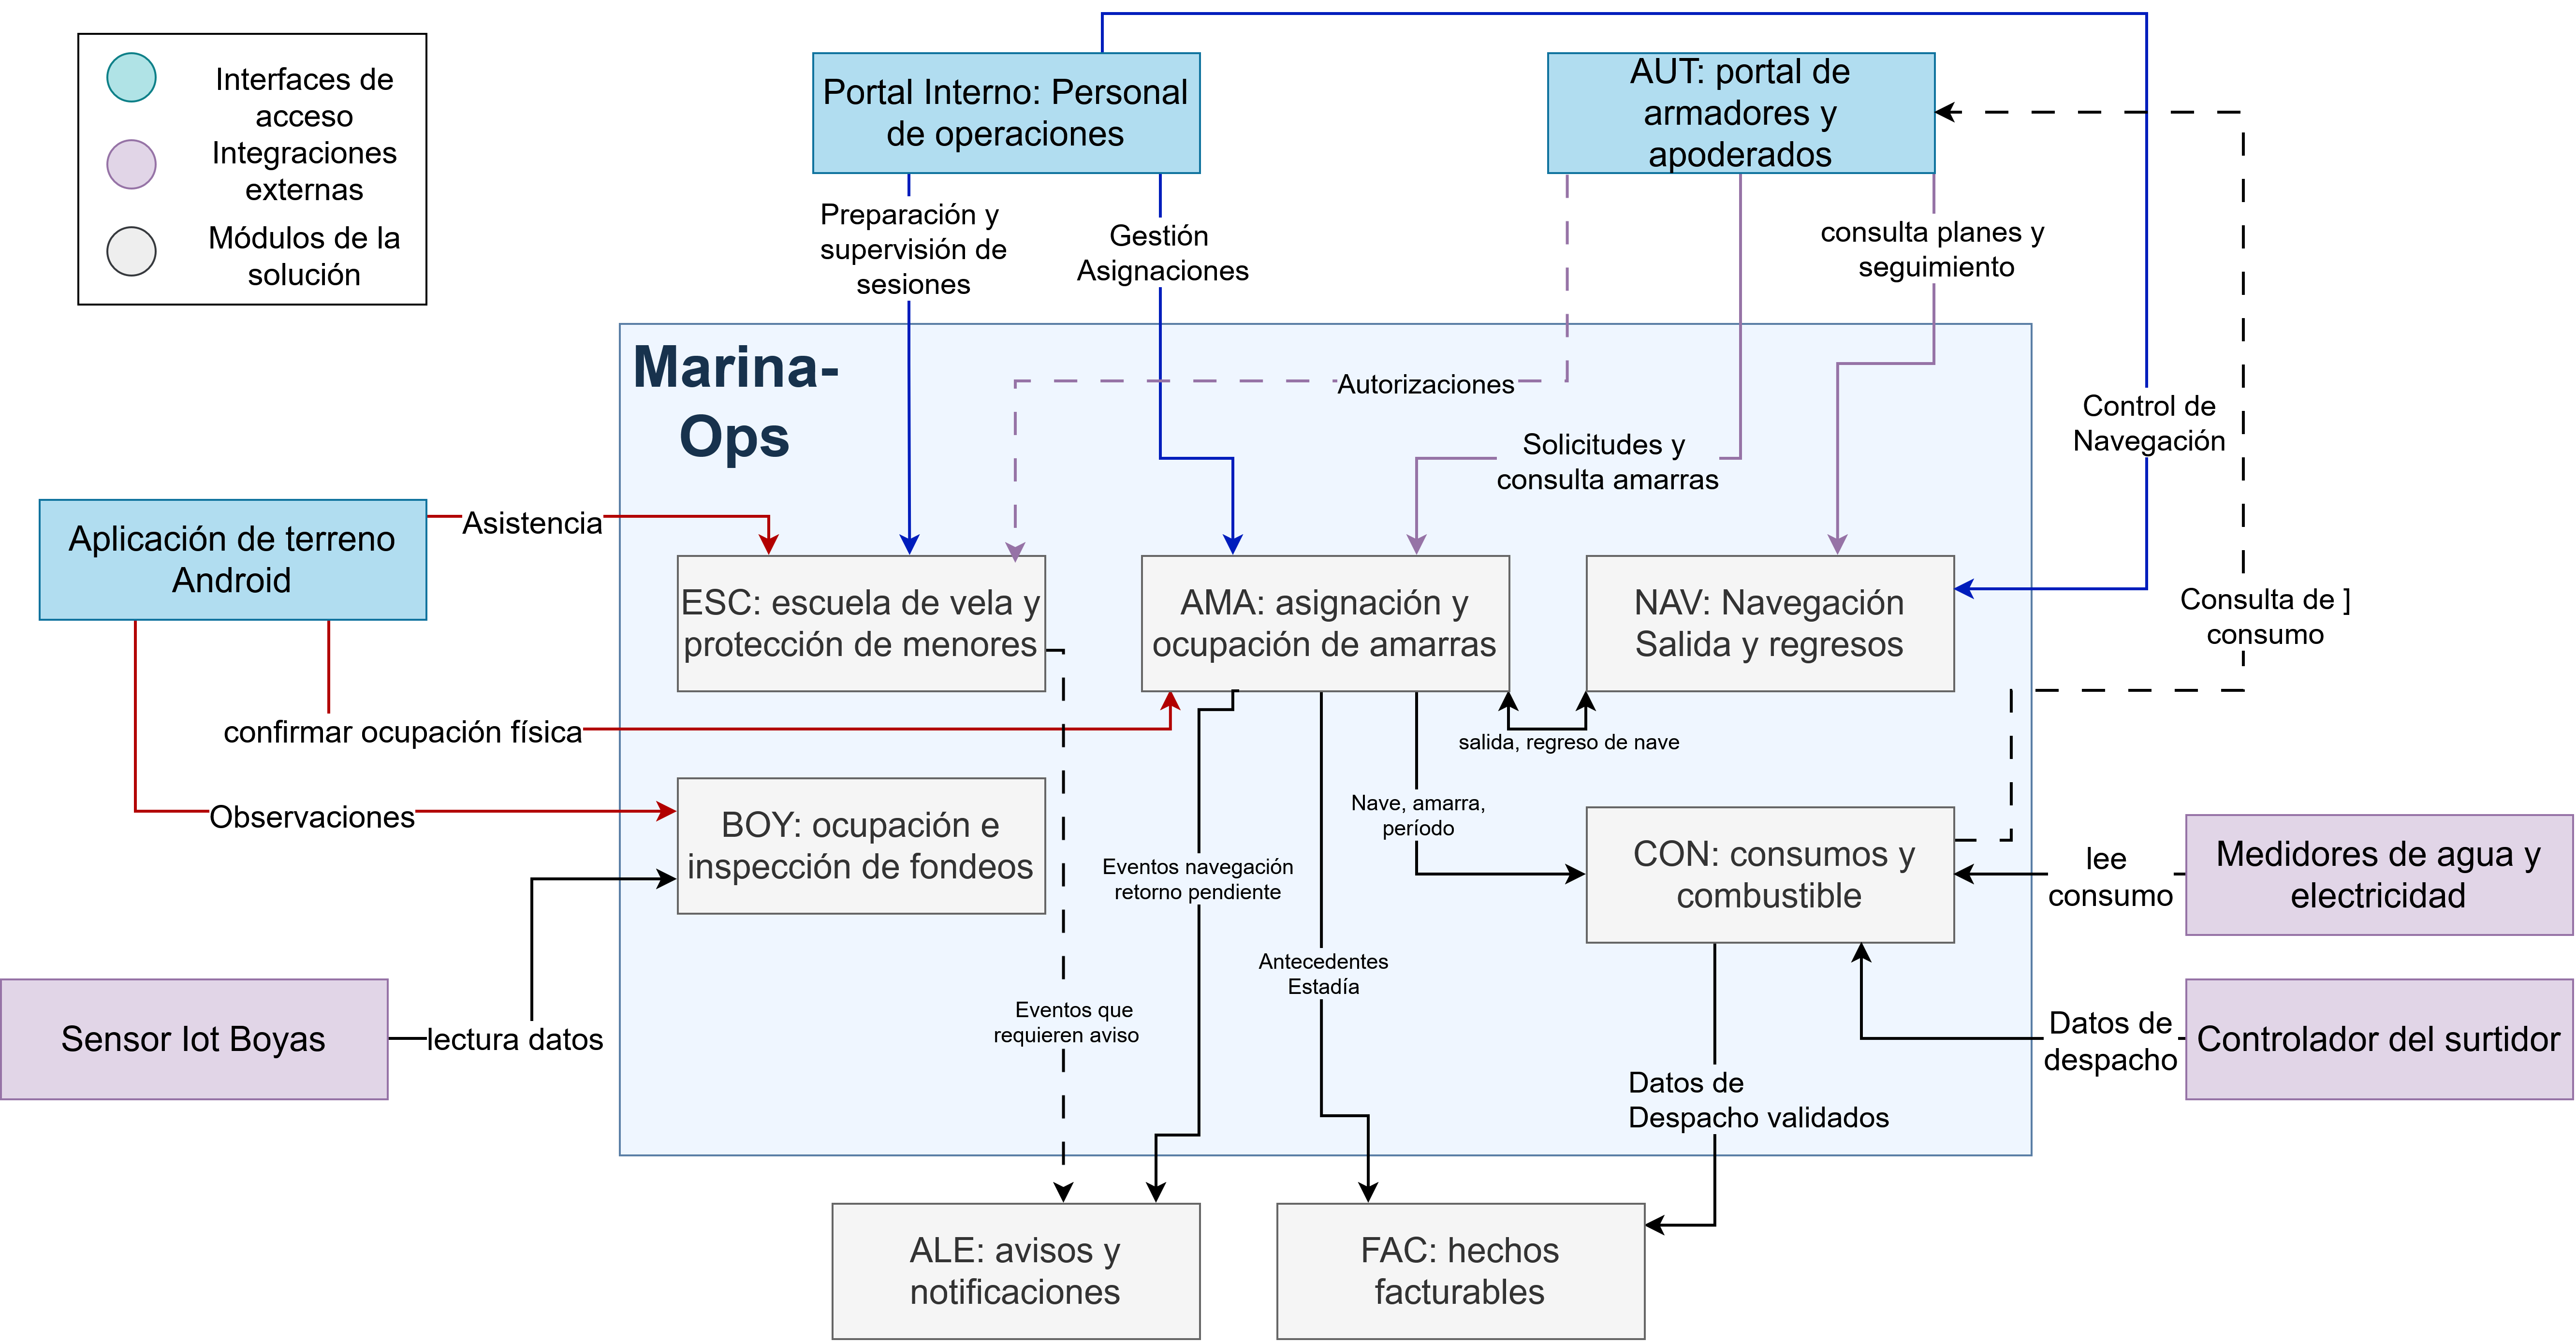
\includegraphics[width=1.15\textwidth]{figuras/diagrama-marina-ops.png}%
    }
    \caption{Descomposición funcional de Marina-Ops y sus intercambios}
    \FuenteTabla{Elaboración propia.}
    \label{fig:descomposicion-marina-ops}
\end{figure}
 Los módulos NAV y AMA relacionan el seguimiento de salidas y regresos con la asignación y ocupación de amarras, permitiendo contrastar los antecedentes declarados con la presencia física de las embarcaciones; una salida no implica liberar automáticamente la amarra, pues su disponibilidad depende de las condiciones contractuales. AMA proporciona a CON la relación entre embarcación, amarra y período de ocupación, necesaria para atribuir los consumos de agua y electricidad recibidos desde los medidores. CON también incorpora los datos del despacho de combustible y, tras su validación, entrega los antecedentes facturables a FAC. Por su parte, ESC reúne la preparación de actividades, las autorizaciones de participación y los registros de asistencia, regreso y entrega de menores, mientras BOY conserva las observaciones de ocupación y las evidencias de inspección de boyas y fondeos. Estas funciones se utilizan mediante tres interfaces complementarias: AUT recibe solicitudes y consultas de usuarios externos, el portal interno permite al personal gestionar la operación y la aplicación de terreno registra las comprobaciones físicas. Los eventos que requieren comunicación se derivan a ALE, mientras ADM proporciona transversalmente identidad, permisos, datos maestros y auditoría. En conjunto, las conexiones permiten mantener la trazabilidad desde la solicitud o lectura inicial hasta su confirmación operacional, notificación o utilización para cobro.


\subsection{Marina-Log: faenas, contratistas y gestión ambiental}

Marina-Log relaciona la organización de faenas con la habilitación
de sus participantes y la evidencia ambiental.
La Figura~\ref{fig:descomposicion-marina-log} distingue
las responsabilidades de VAR, CTR y AMB sin presentar
su proximidad como una secuencia automática.

\begin{figure}[H]
    \centering
    \makebox[\textwidth][c]{%
        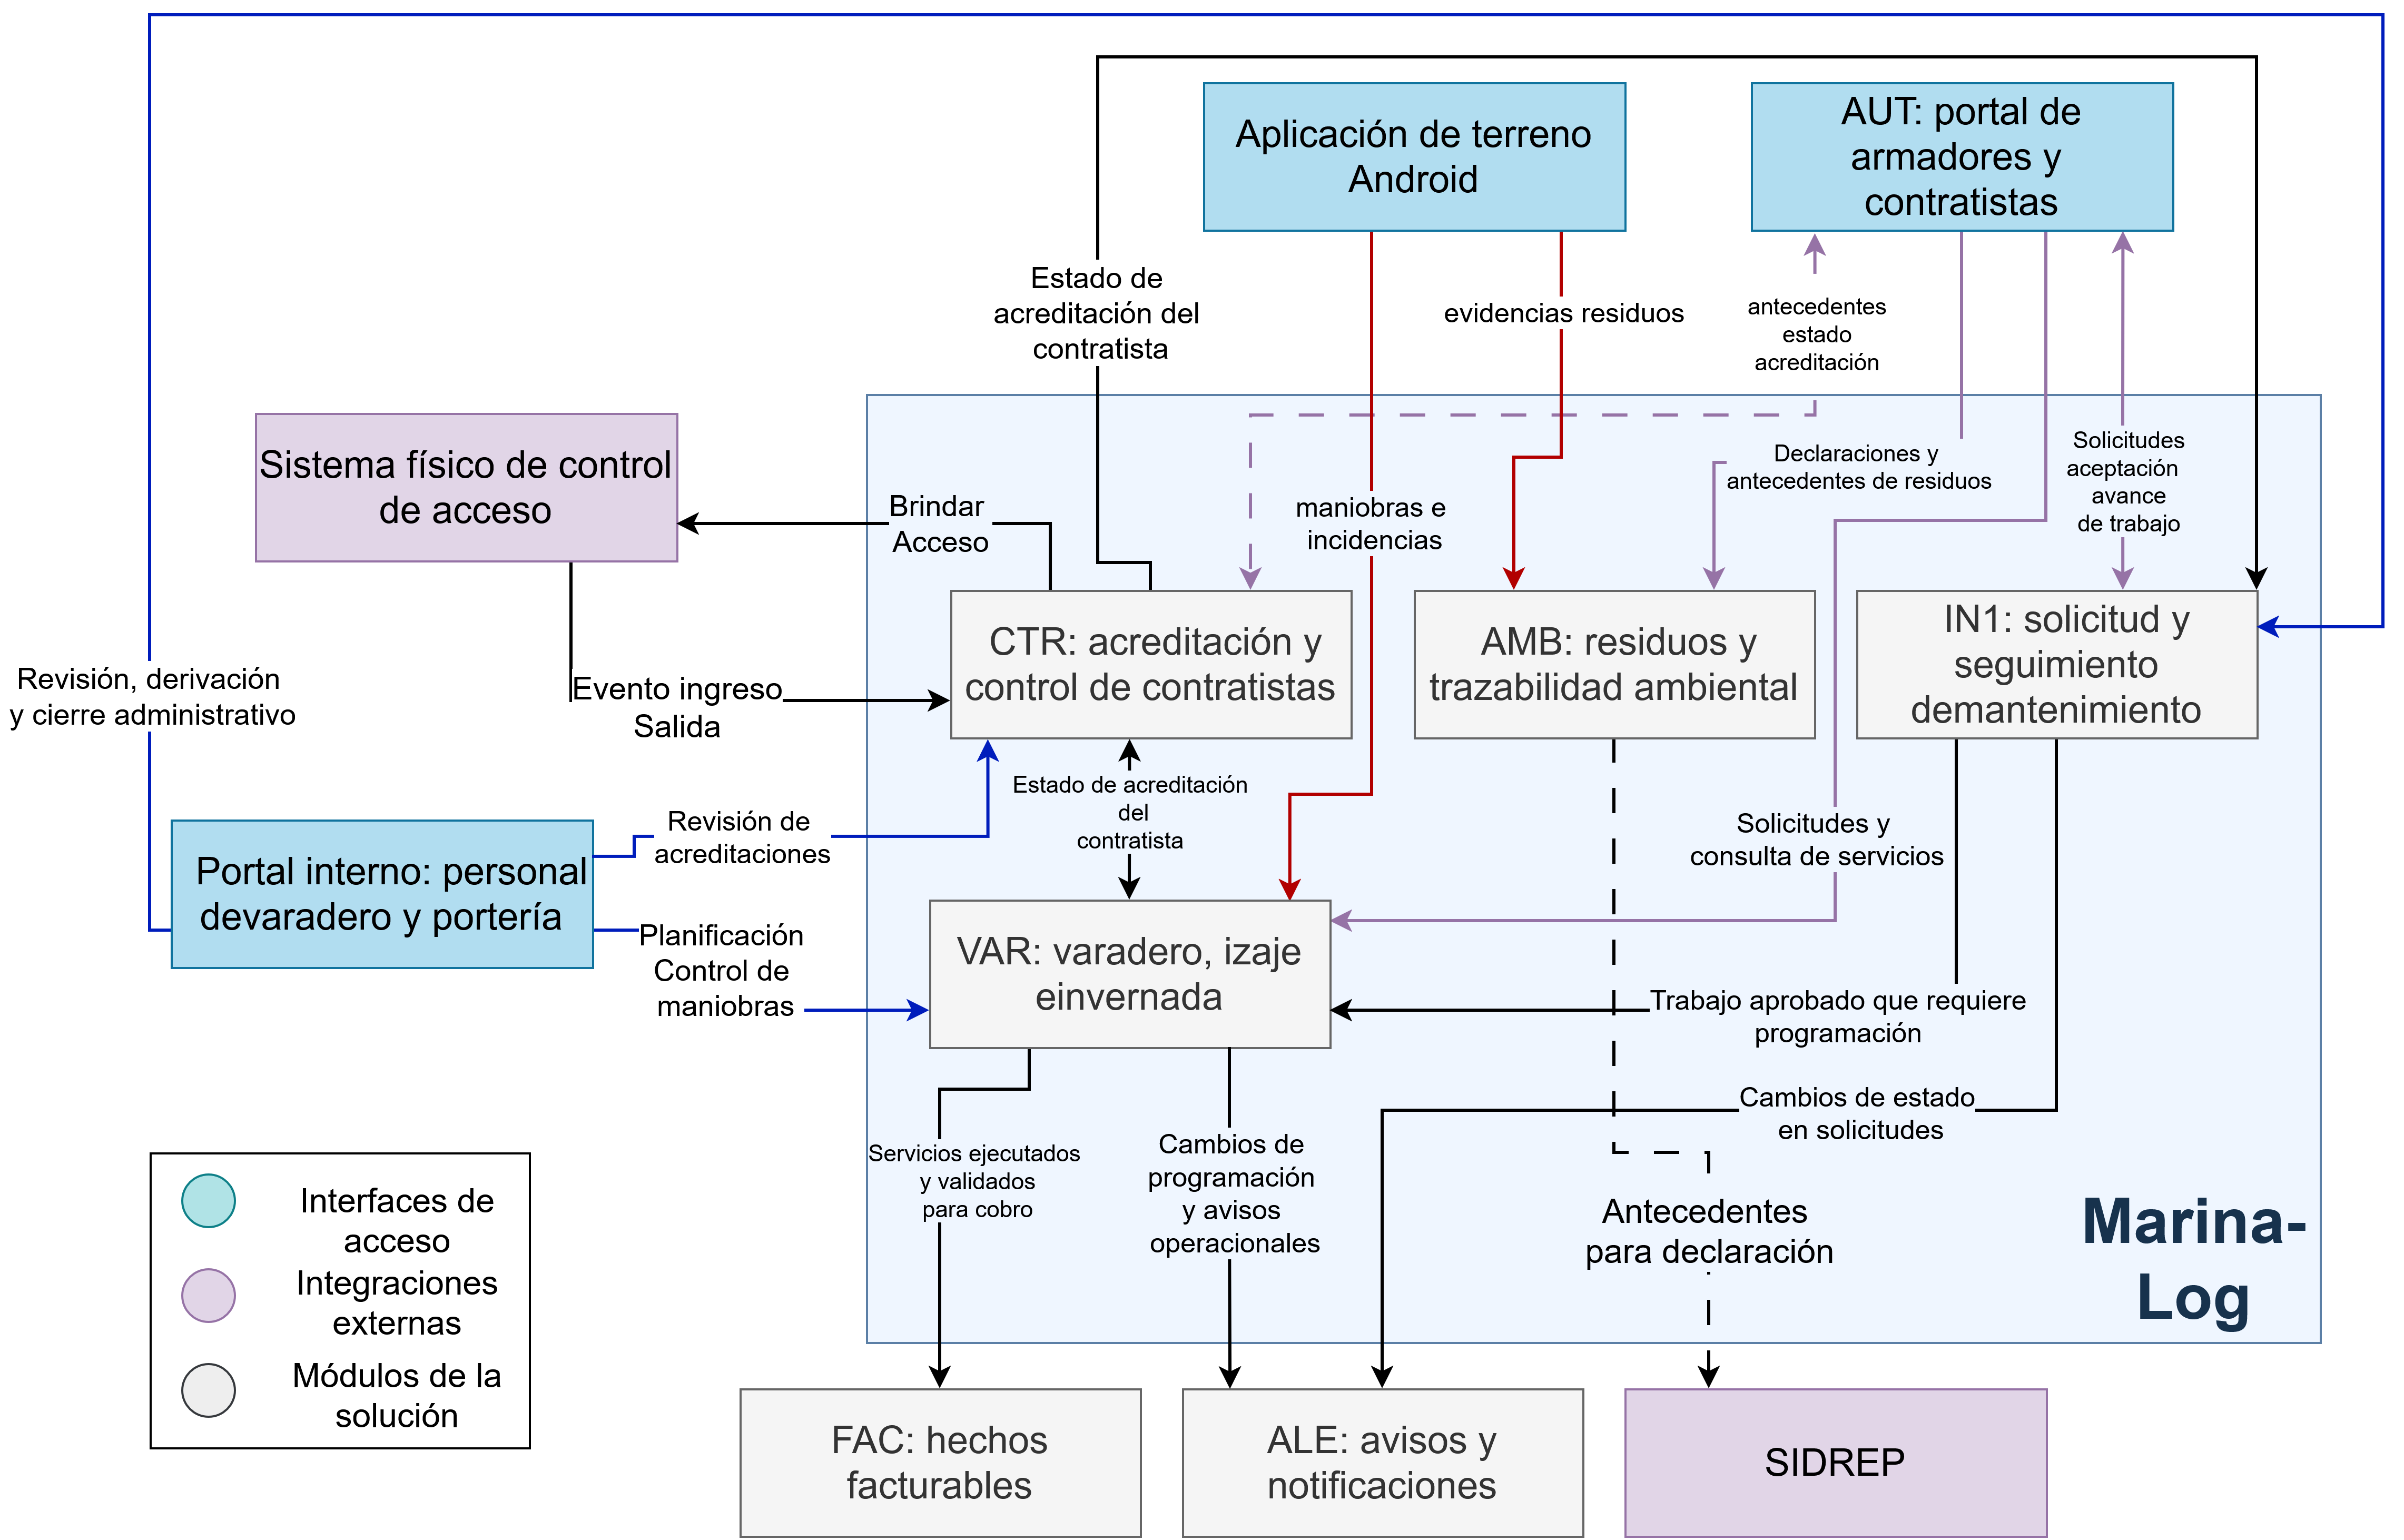
\includegraphics[width=1.1\textwidth]{figuras/diagrama-marina-log.png}%
    }
    \caption{Descomposición funcional de Marina-Log y sus intercambios}
    \label{fig:descomposicion-marina-log}
    \FuenteTabla{Elaboración propia.}
    % Al insertar el diagrama definitivo, incorporar su fuente.
\end{figure}

 VAR concentra la planificación y el registro de maniobras de izaje e invernada, utilizando el estado de acreditación proporcionado por CTR para verificar la habilitación de los contratistas involucrados. CTR se integra con el sistema físico de control de acceso, al que comunica las habilitaciones correspondientes y del que recibe los eventos de ingreso y salida. La Innovación 1 permite registrar solicitudes de mantenimiento, gestionar su revisión y derivación, consultar la aceptación y el avance de los trabajos y efectuar su cierre administrativo; cuando un trabajo aprobado requiere recursos del varadero, se coordina su programación con VAR. La aceptación de la solicitud y la autorización de acceso constituyen decisiones independientes. Por su parte, AMB reúne las declaraciones y evidencias de residuos y prepara los antecedentes para su declaración en SIDREP, conservando la trazabilidad de su gestión. Las interfaces distribuyen la participación según el rol: AUT permite presentar solicitudes y consultar estados, el portal interno concentra la planificación y revisión por el personal autorizado, y la aplicación Android registra maniobras, incidencias y evidencias ambientales en terreno. Finalmente, VAR entrega a FAC los servicios ejecutados y validados para cobro, mientras los cambios de programación y de estado de las solicitudes se comunican a ALE para su notificación. Estos intercambios vinculan cada solicitud con su ejecución, sus responsables y sus antecedentes administrativos y ambientales.


\subsection{Marina-Admin: gestión comercial y atención}

Marina-Admin relaciona hechos operacionales, antecedentes
administrativos y atención externa.
La Figura~\ref{fig:descomposicion-marina-admin} permite seguir
ese intercambio entre FAC, ADM y AUT. ALE aparece agrupado
administrativamente, aunque su alcance comprende las tres unidades.

\begin{figure}[H]
    \centering
    \makebox[\textwidth][c]{%
        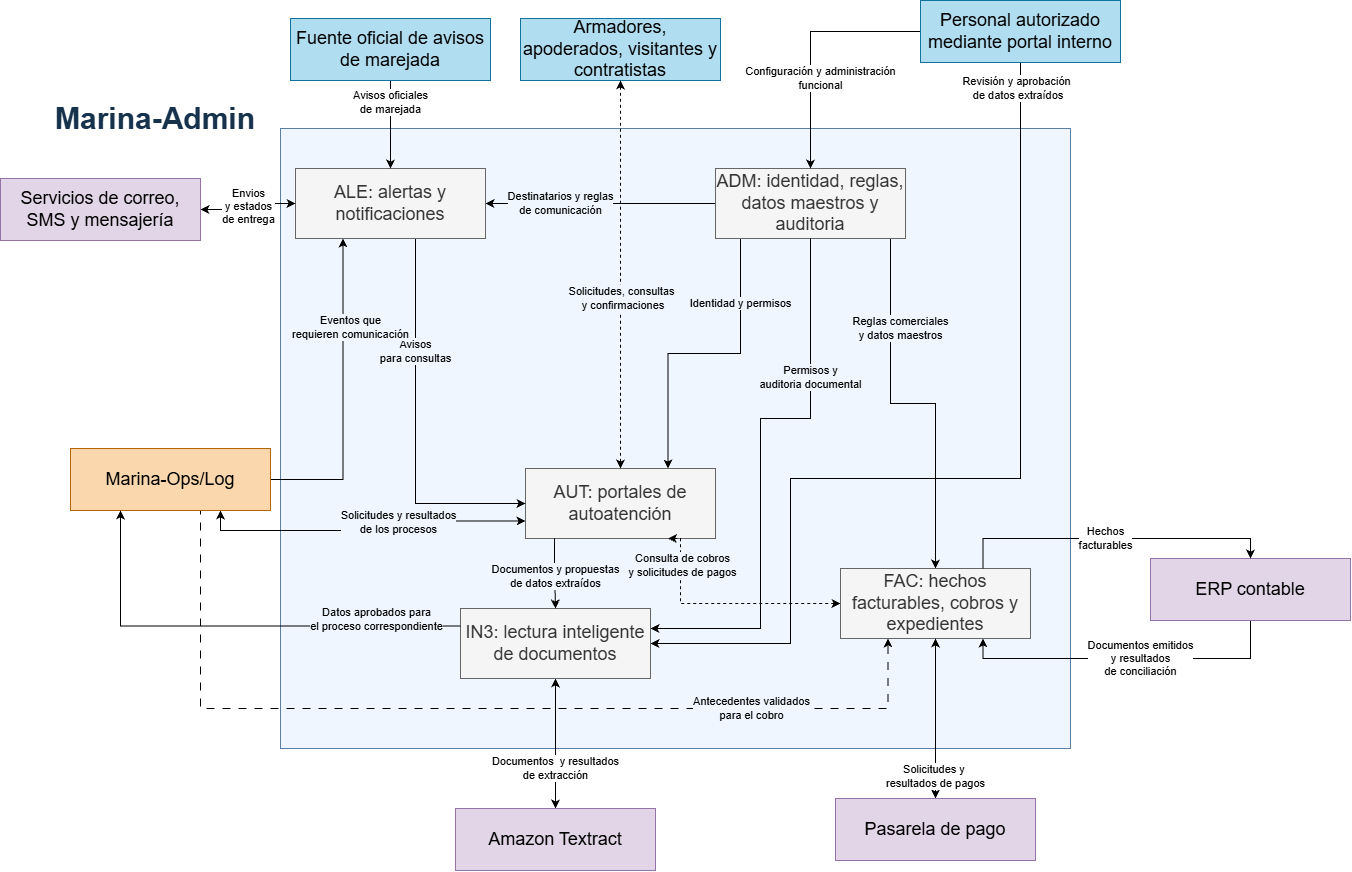
\includegraphics[width=1.15\textwidth]{figuras/diagrama-marina-admin.png}%
    }
    \caption{Descomposición funcional de Marina-Admin y sus intercambios}
    \label{fig:descomposicion-marina-admin}
    \FuenteTabla{Elaboración propia.}
\end{figure}

Marina-Admin concentra las capacidades comerciales y transversales que vinculan la operación de Marina-Ops y Marina-Log con los usuarios y los servicios externos. AUT proporciona un punto de acceso para armadores, apoderados, visitantes y contratistas, canalizando sus solicitudes hacia los módulos responsables y permitiendo consultar los resultados según los permisos definidos por ADM. Este último centraliza la identidad, las reglas configurables, los datos maestros y la auditoría, manteniendo criterios comunes de administración y trazabilidad para toda la plataforma. FAC recibe los antecedentes operacionales validados para cobro y aplica las reglas comerciales correspondientes, conservando la relación entre cada cargo y el servicio o consumo que lo originó. Su integración con el ERP permite comunicar los hechos facturables y recibir los documentos emitidos y los resultados de conciliación, mientras la pasarela de pago proporciona el resultado de las transacciones iniciadas por los usuarios; la emisión tributaria permanece bajo responsabilidad del ERP. ALE reúne los eventos de las unidades operacionales y los avisos oficiales de marejada, utiliza las reglas de destinatarios para distribuir las comunicaciones mediante correo, SMS y mensajería, y registra los estados de entrega. La Innovación 3 complementa estos procesos mediante la lectura inteligente de documentos con Amazon Textract: los resultados de extracción se presentan como propuestas de datos y requieren revisión y aprobación por personal autorizado antes de incorporarse al proceso correspondiente, conservando la alternativa de ingreso manual. De esta forma, la unidad mantiene la continuidad de la información entre solicitudes, operaciones, comunicaciones, documentos y cobros, con responsabilidades diferenciadas y controles comunes.


\subsection{Alertas y canales de interacción}

ALE recibe acontecimientos notificables de las tres unidades y
conserva su relación con destinatarios, canales y resultados.
La guardia incorpora los avisos oficiales de marejada con fuente y
vigencia; los planes vencidos, las comunicaciones escolares,
las reprogramaciones y los vencimientos documentales mantienen sus
responsables funcionales. El aviso no ejecuta por sí mismo la decisión
que comunica ni acredita una actuación física.

Las campañas registran envío, entrega, error y acuse por destinatario,
distinguiendo recepción técnica de confirmación efectiva.
Los contactos sin acuse permiten organizar llamadas y seguimiento;
los datos erróneos originan tareas de corrección.
Las plantillas y preferencias de canal respetan las comunicaciones
obligatorias y las condiciones de baja aplicables.
Los reintentos conservan identidad para evitar efectos duplicados.

La consola apoya la coordinación y administración; AUT atiende
consultas y solicitudes externas; y la aplicación de terreno permite
registrar actuaciones en condiciones seguras.
La radio permanece como medio de coordinación durante maniobras
y contingencias. Una comunicación radial incorporada al sistema
identifica informante, registrador y momento, sin atribuir al canal
evidencia que no haya sido comprobada.


\subsection{Continuidad local y conciliación}

La continuidad conserva las actuaciones críticas cuando se pierde
el enlace exterior y diferencia esa situación del aislamiento
de un terminal. El Nodo de Borde en Recinto sostiene las funciones
locales comprometidas; los dispositivos conservan las capturas
realizadas en terreno. Guardar un registro no equivale
a confirmar una asignación o un retiro escolar.
Cuando no puede comprobarse el estado vigente, se mantiene
la solicitud identificada y se aplica la coordinación segura,
sin presentar información atrasada como autorización.

La conciliación posterior relaciona registros locales y centrales
por su identidad, procedencia y secuencia, evitando duplicados
y conservando discrepancias para su tratamiento trazable.
Esta distinción entre captura, confirmación y conciliación
completa la lectura funcional de los diagramas;
la sección siguiente desarrolla sus recorridos
en situaciones concretas del negocio.


\newpage
\section{Explicación de la Solución}

La solución atiende la dificultad de conocer, compartir
y demostrar el estado de la operación identificada en
el Subdocumento 2. Las vistas de la sección anterior
presentan las responsabilidades funcionales; esta sección
explica cómo colaboran durante la prestación de servicios,
qué decisiones requieren intervención competente y
qué evidencia permite reconstruir sus resultados.

El alcance operacional aquí descrito constituye una referencia para el desarrollo posterior de la arquitectura,
el modelo de datos, los procedimientos y las pruebas.

\subsection{Funcionamiento Operacional y Procesos Críticos de Negocio}

Los recorridos siguientes relacionan una necesidad
de atención con su resultado operacional, administrativo
o ambiental. Distinguen lo solicitado, autorizado y
efectivamente realizado, así como el responsable
que interviene en cada transición. Los antecedentes
se preparan antes de una maniobra y el registro se
completa en condición segura. La radio mantiene
su función de coordinación y no se exige interacción
durante amarre o izaje.

\subsubsection{Recalada, asignación, servicios y cierre comercial}

La atención comienza cuando una embarcación solicita
recalada por un canal admitido o se presenta sin reserva.
AUT canaliza las solicitudes externas y torre incorpora
los antecedentes recibidos por radio. AMA relaciona
dimensiones, características del puesto, disponibilidad
y compromisos existentes antes de confirmar una
asignación. Una salida temporal no libera por sí misma
una amarra permanente. Las excepciones admisibles
requieren la autoridad correspondiente y no permiten
vulnerar condiciones de seguridad.

Durante la estadía se conservan movimientos y servicios
efectivamente registrados. CON relaciona los consumos
con la amarra y el contrato vigente, y mantiene
identificado cada despacho de combustible. VAR aporta
las prestaciones de varadero realizadas. Estos
antecedentes conservan su origen operacional antes
de ser utilizados comercialmente.

FAC comprueba atribución, reglas aprobadas y ausencia
de duplicados antes del intercambio contable.
La respuesta del sistema contable distingue documentos,
pagos y rechazos: enviar antecedentes no acredita
emisión ni pago. El visitante sin prepago mantiene
responsable de pago y estadía registrada, sin condicionar
una maniobra segura a pasar por oficina. Las discrepancias
conservan origen y responsable de revisión.

\subsubsection{Salida, regreso y atención del plan voluntario}

El personal de zarpes utiliza los antecedentes disponibles
para preparar la nómina y el legajo, comprobando vigencias
y faltantes. La Autoridad Marítima conserva el otorgamiento
del zarpe. NAV registra la salida y las personas asociadas
en condición segura. El armador puede declarar o cerrar
un plan mediante AUT, manteniendo su carácter voluntario
y las condiciones de consentimiento; esa declaración
no sustituye el registro operacional.

Al regreso, marinería aporta una observación identificada
de la embarcación amarrada en condición segura. Si se
comunica por radio, se distinguen informante y registrador.
El cierre declarado del plan permanece separado de
esa confirmación, de modo que una diferencia entre
ambos antecedentes continúe visible para su revisión.

Cuando vence un plan sin cierre, ALE genera el aviso
y la guardia registra contactos, resultados y escalamiento
conforme al protocolo autorizado. Un mensaje tardío
se concilia sin borrar la atención realizada ni reabrir
automáticamente un plan cerrado. La marina conserva
evidencia y comunica a los responsables competentes;
no asume funciones de búsqueda o salvamento.

\subsubsection{Participación escolar, entrega y retorno seguro}

ESC relaciona autorizaciones, nómina y asignación
de alumno, bote y monitor antes de la salida.
Los cambios de bote, ausencias y relevos actualizan
la participación efectiva, sin deducirla exclusivamente
de la asistencia inicial. El monitor dispone de
los antecedentes autorizados necesarios para los alumnos
a su cargo, no de acceso indiscriminado a sus expedientes.

Cuando se solicita un retiro, portería comprueba
identidad y autorización del adulto y coordina con
escuela la situación y entrega del alumno. Solicitud,
verificación y entrega confirmada son estados distintos.
Si falla la comunicación, se aplica coordinación segura
y se conserva evidencia de quién informó, verificó
y registró la actuación, sin presentar una copia
atrasada como estado vigente.

El cierre de la clase requiere comprobar a cada
participante. Los casos pendientes permanecen
identificados para seguimiento y no desaparecen
por cerrar administrativamente la actividad.
ALE comunica el resultado seguro al apoderado,
sin cámaras ni seguimiento audiovisual de alumnos.
La consulta se limita al vínculo autorizado con
el alumno correspondiente.

\subsubsection{Faena, habilitación de acceso y trazabilidad de residuos}

VAR organiza la faena y dispone del plan vigente
antes del izaje. El operador calificado valida
sus antecedentes; la aprobación documental no demuestra
que la maniobra haya ocurrido ni constituye un control
físico del equipo. CTR relaciona trabajador, acreditación,
inducción y orden autorizada para que portería compruebe
el acceso.

Los documentos recibidos mediante AUT requieren revisión.
Su presentación o la posesión de una credencial
no autorizan cualquier trabajo. Las excepciones
conservan motivo y responsable, y no sustituyen
las condiciones de seguridad de la actuación.

La ejecución se documenta en momentos seguros,
incluyendo las observaciones del casco cuando
la embarcación está apoyada en tierra. AMB relaciona
los residuos con trabajo, embarcación y generador,
mediante registro directo o asistido. Si el origen
no está acreditado, conserva la recepción y abre
la discrepancia, sin inventar una procedencia.

La entrega al gestor y el certificado posterior
se concilian con el acopio. SIDREP corresponde
a declaración, no a tratamiento material.
Un certificado tampoco resuelve por sí solo
un generador desconocido. El resultado del recorrido
es una cadena de antecedentes que permite distinguir
recepción, traslado y disposición, junto con
las diferencias que todavía requieren aclaración.

\subsubsection{Marejada, inspección de boyas y seguimiento ambiental}

La guardia incorpora el aviso oficial con fuente
y vigencia. ALE organiza la comunicación y diferencia
envío, entrega y acuse, permitiendo seguir contactos
pendientes. Las actividades afectadas se suspenden;
VAR comprueba recursos, posiciones y dependencias
antes de confirmar una nueva agenda y comunicarla.
El aviso no demuestra por sí mismo que todos
los destinatarios hayan ejecutado la actuación indicada.

BOY conserva observaciones e inspecciones identificadas,
su antigüedad y el historial del tren de fondeo.
Contrastar una reserva con una observación permite
detectar discrepancias, no afirmar ocupación actual
sin evidencia. Las inspecciones y actuaciones
se organizan mediante un programa técnico fundamentado,
manteniendo separados el trabajo efectuado
y su registro documental.

Para el seguimiento ambiental, AMB utiliza residuos
trazados y la misma serie validada de consumos de CON.
La evidencia permite revisar las no conformidades
y comprobar qué antecedentes respaldan los indicadores.
Su cierre y la certificación corresponden a
los responsables competentes, no a una declaración
automática de la plataforma.

\subsection{Gobernanza Administrativa, Reglas de Negocio y Gestión de la Información}

La gobernanza distingue la autoridad de negocio de las
tareas técnicas. Los responsables de la marina aprueban
decisiones y validan antecedentes; Synaptix conserva
administración técnica y soporte funcional. ADM reúne
capacidades de configuración y control, pero no sustituye la responsabilidad de NAV, AMA, ESC, CON, BOY, VAR,
CTR, AMB, FAC o AUT sobre sus actuaciones. Los cambios
con impacto operacional mantienen justificación,
versión, aprobaciones y fecha de aplicación.

La propuesta de gobernanza contempla el Registro Local
de Habilitaciones previsto en DEC-22. Gerencia decide
sobre personal propio; Administración registra esas
decisiones mediante titular y suplente delegados.
Los contratistas aportan representantes competentes,
verificados por Varadero. Synaptix aplica la provisión
o baja y conserva su relación con el hecho laboral
que la origina. La falta de comunicación de una decisión exterior durante aislamiento no se presenta como resuelta: se identifica la limitación y la contingencia correspondiente, sin atribuir al cliente una función TI.

La formalización de DEC-22 entregará la matriz de atribuciones, las delegaciones y suplencias, el procedimiento de comunicación de altas y bajas y las reglas de escalamiento del Registro Local de Habilitaciones. El equipo del proyecto preparará el modelo y coordinará su revisión con la contraparte de procesos, que verificará las atribuciones de negocio. Las delegaciones se autorizarán por quienes tengan competencia para otorgarlas. Se comprobarán cargas y cobertura conforme a EST-18 y se ensayará la ausencia del titular antes de habilitar el procedimiento operacional. La evidencia reunirá autorizaciones, procedimientos y resultados de comprobación, para evitar dependencia de una sola persona y mantener separadas la decisión de negocio y su aplicación técnica.

Las reglas propuestas en A2.5 se concretan con las
atribuciones y fundamentos correspondientes.

Los documentos y registros conservan origen, responsable,
versiones y acceso autorizado. Las correcciones no
eliminan silenciosamente antecedentes contradictorios.
FAC relaciona cargos y respuestas contables, y reúne
la evidencia de custodia y abandono para el asesor
autorizado. La integridad del expediente no acredita
por sí sola suficiencia jurídica ni autoriza restricciones
de acceso o actuaciones judiciales.

\subsection{Estrategia de Participación y Adopción de los Grupos de Interés}

Synaptix propone obtener el apoyo de los grupos del Subdocumento~2, sección~2.4, revisando decisiones, comprobando tareas y resolviendo observaciones con registro de su tratamiento. Se organiza la participación según la capacidad de cada actor para decidir o condicionar el proyecto y el efecto del cambio sobre sus actividades. Quienes tienen capacidad de decisión e influencia directa participarán en decisiones y revisiones periódicas. El personal y los usuarios afectados comprobarán tareas y recibirán respuesta a sus observaciones. Con las autoridades y otros actores que intervienen en materias específicas se coordinará la información. Los participantes con intervención limitada recibirán información pertinente y serán consultados cuando una dependencia afecte su servicio. Esta priorización mantendrá los controles de seguridad, la validación de interfaces y suministros, y la representación efectiva de los alumnos.

\subsubsection{Acciones Propuestas por Ámbito de Participación}
La planificación de cada acción identificará a los participantes por los roles indicados, registrará quién representa cada ámbito y coordinará su intervención con el responsable correspondiente. Las designaciones y delegaciones se documentarán por el canal competente. El equipo del proyecto preparará los antecedentes, ejecutará las comprobaciones previstas y conservará las decisiones, observaciones y resultados que constituyen la evidencia de cada acción. Esta organización permite coordinar la participación sin confundir las responsabilidades técnicas con las atribuciones de negocio.

Las actividades incluyen a los participantes de cada bloque, respetando sus funciones y facultades. Las observaciones y correcciones siguen el procedimiento común. Se mantiene el registro en momentos seguros, sin cámaras sobre alumnos ni dispositivos en embarcaciones menores. No se impone seguimiento a bordo ni plan de navegación; el consentimiento es revocable y la deuda no activa bloqueos automáticos.

\paragraph{Gobierno y decisiones}
\mbox{}\par
\noindent Participantes: Directorio, Gerencia y Socios accionistas.

\begin{itemize}
  \setlength{\itemsep}{2pt}
  \setlength{\parsep}{0pt}
  \item Necesidad: decisiones sostenibles, responsabilidades viables y cobranza que afecte el acceso formalmente autorizada.
  \item Acción: revisar atribuciones, delegaciones, alternativas e impactos de discrepancias.
  \item Organización: Jefe de Proyecto de Synaptix y Gerencia; Directorio y Socios accionistas por canal societario.
  \item Momento: gobernanza y antes de cambios relevantes de E1/E2.
  \item Evidencia: decisiones y delegaciones registradas.
\end{itemize}

\paragraph{Operación náutica y terreno}
\mbox{}\par
\noindent Participantes: Jefatura de operaciones, Torre de control, Marineros de pantalán, Personal de combustible y Mantenimiento e inspección de boyas.

\begin{itemize}
  \setlength{\itemsep}{2pt}
  \setlength{\parsep}{0pt}
  \item Necesidad: estados confiables y registro seguro sin enlace exterior.
  \item Acción: ensayar salidas/regresos, avisos, despacho e inspección con comunicación limitada y registro en momentos seguros.
  \item Organización: equipo funcional de Synaptix y Jefatura de operaciones.
  \item Momento: diseño y marcha blanca de E1; cambios pertinentes de E2.
  \item Evidencia: procedimientos revisados y tareas comprobadas.
\end{itemize}

\paragraph{Varadero e izaje}
\mbox{}\par
\noindent Participantes: Responsable de varadero y Operadores de travelift.

\begin{itemize}
  \setlength{\itemsep}{2pt}
  \setlength{\parsep}{0pt}
  \item Necesidad: programación y evidencia compatibles con el izaje seguro.
  \item Acción: revisar plan, reprogramación y registro previo/posterior, fuera de izajes activos.
  \item Organización: equipo funcional de Synaptix y Responsable de varadero; operadores comprueban el uso práctico.
  \item Momento: diseño y marcha blanca de E2, en ventanas permitidas.
  \item Evidencia: procedimiento validado por roles competentes.
\end{itemize}

\paragraph{Coordinación escolar}
\mbox{}\par
\noindent Participantes: Coordinación de escuela de vela, Monitores de escuela de vela y Portería y seguridad.

\begin{itemize}
  \setlength{\itemsep}{2pt}
  \setlength{\parsep}{0pt}
  \item Necesidad: autorizaciones, cambios, retiros y regreso coherentes con la participación efectiva de cada alumno.
  \item Acción: simular retiro durante clase, cambio de bote, relevo de monitor, interrupción de comunicación y alumno pendiente; verificar quién comprueba y registra.
  \item Organización: equipo funcional de Synaptix y Coordinación de escuela de vela.
  \item Momento: diseño y marcha blanca de E1; cambios posteriores.
  \item Evidencia: procedimiento de entrega/regreso y escenarios comprobados.
\end{itemize}

\paragraph{Representación de alumnos y apoderados}
\mbox{}\par
\noindent Participantes: Apoderados, Centro de padres y Alumnos de la escuela.

\begin{itemize}
  \setlength{\itemsep}{2pt}
  \setlength{\parsep}{0pt}
  \item Necesidad: seguridad, comunicación confiable y acceso limitado a datos de menores.
  \item Acción: revisar autorizaciones, retiro e información; escuela y apoderados representan a los alumnos, sin exigirles aprobar el proyecto.
  \item Organización: Synaptix prepara; Coordinación de escuela de vela convoca con apoderados y Centro de padres.
  \item Momento: antes de cerrar el diseño escolar de E1 y en su marcha blanca.
  \item Evidencia: observaciones con respuesta fundada y ajustes comprobados.
\end{itemize}

\paragraph{Gestión administrativa}
\mbox{}\par
\noindent Participantes: Administración, Atención a socios y Gestión de cobranza (administración).

\begin{itemize}
  \setlength{\itemsep}{2pt}
  \setlength{\parsep}{0pt}
  \item Necesidad: cargos respaldados, diferencias resueltas y seguimiento de deuda dentro de las atribuciones autorizadas.
  \item Acción: revisar servicios, consumos, duplicados y discrepancias contables; distinguir atención, consolidación y cobranza.
  \item Organización: equipo funcional de Synaptix y Administración.
  \item Momento: datos y responsabilidades en E1; diseño y marcha blanca comercial de E2.
  \item Evidencia: reglas revisadas, casos conciliados y procedimiento de discrepancias.
\end{itemize}

\paragraph{Atención a usuarios}
\mbox{}\par
\noindent Participantes: Armadores, Socios del club y Visitantes y tripulaciones.

\begin{itemize}
  \setlength{\itemsep}{2pt}
  \setlength{\parsep}{0pt}
  \item Necesidad: atención ágil, servicios/cargos revisables, comunicación clara y privacidad de navegación.
  \item Acción: comprobar solicitudes, estados y avisos; consentimiento y retiro del plan voluntario con armadores; canales e idiomas con visitantes y tripulaciones.
  \item Organización: Synaptix, Atención a socios y Jefatura de operaciones; convocatoria acordada con la marina.
  \item Momento: antes de habilitar funciones de E1/E2 y en sus marchas blancas.
  \item Evidencia: instrucciones revisadas y tareas comprobadas.
\end{itemize}

\paragraph{Operadora de charter}
\mbox{}\par
\noindent Participantes: Operadora de charter.

\begin{itemize}
  \setlength{\itemsep}{2pt}
  \setlength{\parsep}{0pt}
  \item Necesidad: continuidad comercial y evidencia de servicios y condiciones documentados en SD2.
  \item Acción: revisar atribución de consumos, atención, evidencia ambiental y diferencias respecto de las condiciones documentadas.
  \item Organización: Synaptix, Gerencia y Administración, con representante de la operadora.
  \item Momento: evidencia en E1; revisión comercial/ambiental en E2 y seguimiento hacia 2029.
  \item Evidencia: antecedentes revisados y observaciones tratadas.
\end{itemize}

\paragraph{Contratistas}
\mbox{}\par
\noindent Participantes: Empresas contratistas y Trabajadores de contratistas.

\begin{itemize}
  \setlength{\itemsep}{2pt}
  \setlength{\parsep}{0pt}
  \item Necesidad: acreditación de acceso/trabajos y origen de residuos sin depender del uso generalizado de una aplicación.
  \item Acción: ensayar acreditación, declaración y captura directa o asistida autorizada; comprobar origen, revisión y discrepancias, manteniendo portal y declaración.
  \item Organización: Synaptix, Responsable de varadero y Portería y seguridad.
  \item Momento: diseño y marcha blanca de E2, antes de exigir el procedimiento.
  \item Evidencia: procedimiento practicable y capacitación registrada.
\end{itemize}

\paragraph{Trazabilidad ambiental}
\mbox{}\par
\noindent Participantes: Gestor autorizado de residuos, Certificador ambiental y Autoridad sanitaria.

\begin{itemize}
  \setlength{\itemsep}{2pt}
  \setlength{\parsep}{0pt}
  \item Necesidad: evidencia de recepción, destino y antecedentes ambientales.
  \item Acción: contrastar entregas/certificados con el gestor, documentación con el certificador y consultas oficiales con la autoridad sanitaria.
  \item Organización: Synaptix prepara; Gerencia y Responsable de varadero coordinan por separado con cada tercero.
  \item Momento: consumos en E1; residuos en E2 y seguimiento previo a la temporada 2029.
  \item Evidencia: formatos contrastados, consultas registradas y respuestas recibidas incorporadas; pendientes identificados.
\end{itemize}

\paragraph{Coordinación marítima y aseguradoras}
\mbox{}\par
\noindent Participantes: Autoridad marítima y Aseguradoras.

\begin{itemize}
  \setlength{\itemsep}{2pt}
  \setlength{\parsep}{0pt}
  \item Necesidad: antecedentes de zarpe y avisos, y documentación de incidentes y cobertura, según competencia.
  \item Acción: consultar antecedentes de zarpe y avisos con la autoridad marítima por canal oficial; revisar incidentes y maniobras separadamente con aseguradoras.
  \item Organización: Synaptix y Jefatura de operaciones o Responsable de varadero preparan; Gerencia coordina cada consulta.
  \item Momento: diseño de E1/E2, antes de cerrar procedimientos.
  \item Evidencia: consultas y respuestas registradas y requisitos documentales precisados.
\end{itemize}

\paragraph{Suministros e integraciones}
\mbox{}\par
\noindent Participantes: Concesionario del restaurante, Proveedores de servicios e infraestructura y Responsables de sistemas que se mantienen.

\begin{itemize}
  \setlength{\itemsep}{2pt}
  \setlength{\parsep}{0pt}
  \item Necesidad: antecedentes contractuales/consumos, condiciones de suministro e interfaces compatibles.
  \item Acción: revisar consumos del restaurante, suministros habituales/específicos y formatos, restricciones e intercambios de sistemas conservados.
  \item Organización: Synaptix coordina las especificaciones e interfaces y Administración los antecedentes de negocio. Antes de especificar, adquirir o integrar cada dependencia, se identificarán y registrarán los interlocutores del concesionario, de los proveedores y de los sistemas conservados, junto con su ámbito de responsabilidad, para resolver las condiciones de suministro e intercambio con los participantes correspondientes.
  \item Momento: antes de especificar, adquirir o integrar cada dependencia de E1/E2.
  \item Evidencia: condiciones y formatos documentados y dependencias comprobadas.
\end{itemize}

\subsubsection{Seguimiento de Observaciones y Comprobación de Adopción}

Cada observación registrará grupo/rol de origen, proceso, necesidad, responsable de respuesta, decisión, fundamento y evidencia de cierre. Synaptix propondrá incorporar, ajustar o descartar la solicitud con fundamento; el responsable de negocio resolverá dentro de sus atribuciones. Un acuerdo mayoritario no podrá eliminar restricciones de seguridad, privacidad o de las bases.

En las marchas blancas se observarán tareas, dificultades y uso de contingencias, y se registrará la capacitación realizada. Asistir a una sesión o recibir una comunicación no demuestra adopción. Las dificultades exigirán ajustes y nueva comprobación antes del hito correspondiente, sin desplazar automáticamente hitos contractuales.

La participación de los grupos de interés comprende la revisión de decisiones de negocio, la comprobación de tareas, la capacitación y el tratamiento de observaciones durante la implementación e implantación. Su programación y los recursos asociados se incorporarán al Subdocumento~7, respetando el congelamiento del 15 de diciembre al 15 de marzo, las campañas de varadero, el calendario náutico y las suspensiones por marejada, para evitar interferencias con las operaciones y actividades de riesgo.

Durante la operación, el proveedor conserva la administración técnica y el soporte funcional, mientras los responsables de negocio mantienen las decisiones y autorizaciones propias de sus atribuciones. La planificación contemplará el esfuerzo de participación y las tareas recurrentes vinculadas a EST-18. Esta separación permite organizar la intervención del cliente sin trasladarle funciones de tecnologías de información.

La estrategia entregará el registro de decisiones y procedimientos revisados, las observaciones de los participantes con su tratamiento fundamentado y la evidencia de capacitación y comprobación de tareas. Estos antecedentes permitirán verificar la preparación de cada grupo para las funciones que utilizará y orientar los ajustes antes del hito correspondiente. Su revisión formará parte del expediente de implantación; la aceptación contractual se formalizará mediante los actos de recepción previstos. Las autorizaciones, fiscalizaciones y certificaciones conservarán los procedimientos y competencias de las autoridades y terceros correspondientes.


\subsection{Criterios de Experiencia de Usuario y Operación en Cubierta}

Las interfaces deben permitir reconocer la tarea,
el antecedente utilizado y el resultado alcanzado
en las condiciones reales del recinto. El registro
se organiza alrededor del momento seguro; no exige
interacción con cabos en tensión o carga suspendida.
Se comprobará su utilización con guantes,
pantalla mojada, exposición solar y comunicación
limitada, sin considerar demostrado el desempeño
por el tamaño de un control gráfico.

La presentación distingue registro conservado,
solicitud pendiente y actuación confirmada.
Una vista atrasada no autoriza exclusivamente
un puesto ni confirma un retiro escolar.
La identidad individual y la habilitación vigente
permanecen reconocibles aunque el dispositivo
sea compartido por turno. Ante imposibilidad
de comprobar una condición necesaria, se explica
qué no puede confirmarse y cómo continuar mediante
el procedimiento seguro.

Las consultas y comunicaciones respetan accesibilidad
y los idiomas exigidos para visitantes y tripulaciones.
Los avisos expresan el resultado comprobado,
evitando ambigüedades entre una solicitud recibida
y una actuación realizada.
